% Impostazioni principali
\documentclass[t, compress, mathserif]{beamer}



%         ----------------------------------------------         %
%        /                                              \        %
%--------               START PREAMBLE                   --------%
%        \                                              /        %
%         ----------------------------------------------         %

% Titolo che appare nella prima slide del documento
\newcommand{\titolo}{Inferential Statistics}
\newcommand{\sottotitolo}{}

% Titolo che appare nella barra in basso di ogni slide, al centro
% Sono due variabili:
% * una puo' essere utilizzata per l'intero corso. Se impostata nel preambolo sovrascrive quella di seguito.
% * l'altra puo' identificare ciascun documento
\newcommand{\titolocompleto}{Statistics Course - }
\newcommand{\titoloshort}{\titolo}

% Numero di capitolo o altro nome che appare in basso di ogni slide, vicino al numero di pagina
\newcommand{\numerocapitolo}{Chapter 3}

% Include il documento che contiene il preambolo

%%%%%%%%%%%%%%%%%%%%%%%%%%%%%%%%%%%%%%%%%%%%%%%%%%%%%%%%%%%%%%%%%%%%%%%%%%%%%%
%%%%%%%%%%%%%%%%%%%%%%%%%%%% VARIABILI DA DEFINIRE %%%%%%%%%%%%%%%%%%%%%%%%%%%
%%%%%%%%%%%%%%%%%%%%%%%%%%%%%%%%%%%%%%%%%%%%%%%%%%%%%%%%%%%%%%%%%%%%%%%%%%%%%%

% Titolo che appare nella barra in basso di ogni slide, al centro
% Se impostato ha la precedenza rispetto a quello di ogni singola slide

%\renewcommand{\titolocompleto}{}

% non c'e' newcommand{\sottotitolo} perche' viene definito in ogni slide
\newcommand{\data}{}



%%%%%%%%%%%%%%%%%%%%%%%%%%%%%%%%%%%%%%%%%%%%%%%%%%%%%%%%%%%%%%%%%%%%%%%%%%%%%%
%%%%%%%%%%%%%%%%%%%%%%%%%%%%%%%%%% PACKAGES %%%%%%%%%%%%%%%%%%%%%%%%%%%%%%%%%%
%%%%%%%%%%%%%%%%%%%%%%%%%%%%%%%%%%%%%%%%%%%%%%%%%%%%%%%%%%%%%%%%%%%%%%%%%%%%%%
\usepackage[latin1]{inputenc}   
\usepackage{graphicx}
\usepackage{rotating}
\usepackage{rotfloat}
\usepackage{color}
\usepackage{colortbl}
\usepackage{../includeTex/floatflt}
\usepackage{tikz}
\usepackage{hyperref}
\usepackage{pgfpages} 
\usepackage{ifthen}
\usepackage{wasysym}
\usepackage{multirow}



%%%%%%%%%%%%%%%%%%%%%%%%%%%%%%%%%%%%%%%%%%%%%%%%%%%%%%%%%%%%%%%%%%%%%%%%%%%%%%
%%%%%%%%%%%%%%%%%%%%%%%%%%%% IMPOSTAZIONI GENERALI %%%%%%%%%%%%%%%%%%%%%%%%%%%
%%%%%%%%%%%%%%%%%%%%%%%%%%%%%%%%%%%%%%%%%%%%%%%%%%%%%%%%%%%%%%%%%%%%%%%%%%%%%%

% Beamer theme
%\usetheme{CambridgeUS}      
\usetheme{Madrid}      

% Immagini da visualizzare
\newcommand{\materiale}{minitab}

% Path delle immagini
\graphicspath{{../images/}}

% Per caricare le formule matematiche con il giusto font 
% Questo sostituisce l'opzione mathserif di documentclass (obsoleta) 
\usefonttheme[onlymath]{serif}      

     

%%%%%%%%%%%%%%%%%%%%%%%%%%%%%%%%%%%%%%%%%%%%%%%%%%%%%%%%%%%%%%%%%%%%%%%%%%%%%%
%%%%%%%%%%%%%%%%%%%%%%%%%%%%%%%%%%% COLORI %%%%%%%%%%%%%%%%%%%%%%%%%%%%%%%%%%%
%%%%%%%%%%%%%%%%%%%%%%%%%%%%%%%%%%%%%%%%%%%%%%%%%%%%%%%%%%%%%%%%%%%%%%%%%%%%%%

\definecolor{grigio}{rgb}{0.46,0.48,0.48}
\definecolor{giallo}{rgb}{1,0.84,0}
\definecolor{coolred}{rgb}{0.83,0.06,0.27}
\definecolor{arancio}{rgb}{0.97,0.46,0.09}
\definecolor{verde}{rgb}{0.25,0.78,0.25}
\definecolor{qblu}{rgb}{0.24,0.27,0.74}
\definecolor{azzurro}{rgb}{0.37,0.91,0.90}

\definecolor{grigio}{rgb}{0.46,0.48,0.48}
\definecolor{blu}{rgb}{0.25,0.28,0.78}

\definecolor{sfondoScopo}{rgb}{0.75,0.785,0.83}
\definecolor{darkred}{named}{qblu}
\definecolor{blue}{named}{qblu}

\setbeamercolor{scopo}{bg=sfondoScopo}
\setbeamercolor{section in toc}{fg=black,bg=white}
\setbeamercolor{alerted text}{fg=darkred!80!gray}
\setbeamercolor{palette primary}{fg=darkred!60!black,bg=gray!30!white}
\setbeamercolor{palette secondary}{fg=darkred!70!black,bg=gray!15!white}
\setbeamercolor{palette tertiary}{bg=darkred!80!black,fg=gray!10!white}
\setbeamercolor{palette quaternary}{fg=darkred,bg=gray!5!white}

\setbeamercolor{sidebar}{fg=darkred,bg=gray!15!white}
\setbeamercolor{palette sidebar primary}{fg=darkred!10!black}
\setbeamercolor{palette sidebar secondary}{fg=white}
\setbeamercolor{palette sidebar tertiary}{fg=darkred!50!black}
\setbeamercolor{palette sidebar quaternary}{fg=gray!10!white}

\setbeamercolor{titlelike}{parent=pallette primary,fg=darkred}
\setbeamercolor{frametitle}{bg=gray!10!white}
\setbeamercolor{frametitle right}{bg=gray!60!white}

\setbeamercolor{separation line}{}
\setbeamercolor{fine separation line}{}

%% Definizione dei colori da assegnare ai box
\setbeamercolor{postit}{fg=white,bg=qblu}
\setbeamercolor{postut}{fg=qblu,bg=gray!60!white}

%% Definizione dei colori per i diagrammi
\definecolor{bloccoIniziale}{rgb}{0.94,0.93,0.48}
\definecolor{bloccoFinale}{rgb}{0.86,0.25,0.27}
\definecolor{blocco}{rgb}{0.56,0.58,0.77}
\definecolor{bloccoSospeso}{rgb}{0.94,0.81,0.36}



%%%%%%%%%%%%%%%%%%%%%%%%%%%%%%%%%%%%%%%%%%%%%%%%%%%%%%%%%%%%%%%%%%%%%%%%%%%%%%
%%%%%%%%%%%%%%%%%%%%%%%%% STRUTTURA DELLE DIAPOSITIVE %%%%%%%%%%%%%%%%%%%%%%%%
%%%%%%%%%%%%%%%%%%%%%%%%%%%%%%%%%%%%%%%%%%%%%%%%%%%%%%%%%%%%%%%%%%%%%%%%%%%%%%

% Intestazione
\setbeamertemplate{headline}
{
  \leavevmode%
  \hbox{%
  \begin{beamercolorbox}[wd=.5\paperwidth,ht=2.25ex,dp=1ex,right]{section in head/foot}%
    \usebeamerfont{section in head/foot}\insertsectionhead\hspace*{2ex}
  \end{beamercolorbox}%
  \begin{beamercolorbox}[wd=.5\paperwidth,ht=2.25ex,dp=1ex,left]{subsection in head/foot}%
    \usebeamerfont{subsection in head/foot}\hspace*{2ex}\insertsubsectionhead
  \end{beamercolorbox}}%
  \vskip0pt%
}

% Pie' di pagina
\setbeamertemplate{footline}
{
  \hbox{%
    \begin{beamercolorbox}[wd=.20\paperwidth, ht = 2.25ex, dp = 1ex, center]{palette sidebar secondary}%
      \usebeamerfont{author in head/foot}%\insertshortauthor~~(\insertshortinstitute) 
      
\includegraphics[width=1.5cm]{QUANTIDE.jpg}
    \end{beamercolorbox}%
    \begin{beamercolorbox}[wd=.57\paperwidth, ht = 2.25ex, dp = 1ex, center]{title in head/foot}%
      \usebeamerfont{title in head/foot}{\titolocompleto \titoloshort}
    \end{beamercolorbox}%
    \begin{beamercolorbox}[wd=.13\paperwidth, ht = 2.25ex, dp = 1ex, left]{date in head/foot}%
      \hspace*{0.4em} \usebeamerfont{date in head/foot} {\numerocapitolo}
    \end{beamercolorbox}%
    \begin{beamercolorbox}[wd=.10\paperwidth, ht = 2.25ex, dp = 1ex, right]{date in head/foot}%
       \usebeamerfont{date in head/foot} \insertframenumber{} / \inserttotalframenumber \hspace*{2ex} 
    \end{beamercolorbox}%
  }%
  \vskip0pt%
}



%%%%%%%%%%%%%%%%%%%%%%%%%%%%%%%%%%%%%%%%%%%%%%%%%%%%%%%%%%%%%%%%%%%%%%%%%%%%%%
%%%%%%%%%%%%%%%%%%%%%%%%%%% STILE DELLE DIAPOSITIVE %%%%%%%%%%%%%%%%%%%%%%%%%%
%%%%%%%%%%%%%%%%%%%%%%%%%%%%%%%%%%%%%%%%%%%%%%%%%%%%%%%%%%%%%%%%%%%%%%%%%%%%%%

% Simboli di navigazione
\setbeamertemplate{navigation symbols}{}

% Modifica lo stile dell'elenco (di primo livello)
\useitemizeitemtemplate{$\star$} % Usa la stella

% Interlinea (fattore di scala; NON e' un valore assoluto)
\renewcommand{\baselinestretch}{1.2}  

% Definisci stile per vettori e matrici
\newcommand{\vect}[1]{\boldsymbol{\underline{#1}}} % Grassetto e sottolineato
\newcommand{\matr}[1]{\boldsymbol{#1}} % Grassetto

% Definire stile per valore assoluto
\providecommand{\abs}[1]{\lvert#1\rvert}
\providecommand{\norm}[1]{\lVert#1\rVert}

% Cambiare il nome delle figure e delle tabelle
\renewcommand{\figurename}{Figura}
\renewcommand{\tablename}{Tabella}

% Definizione sezioni, ecc.
\newcommand{\livelloA}{\section}
\newcommand{\livelloB}{\subsection}
\newcommand{\livelloC}{\subsubsection}

% Livello di profondita' del 'content panel' del PDF
% \hypersetup{bookmarksdepth=4} % il valore di default va bene

% Definizione prima slide
\title{\textbf{\titolo}}
\author{\sottotitolo}
\date{\data}






%         ----------------------------------------------         %
%        /                                              \        %
%--------               START DOCUMENT                   --------%
%        \                                              /        %
%         ----------------------------------------------         %

\begin{document}

% Pagina del titolo
\frame{\titlepage}

% Indice
% \begin{frame}
% 	 \tableofcontents
% \end{frame}

% Documento
% I soli contenuti del documento sono in un file esterno. Questo semplifica enormemente le cose qualora si volessero creare dei manuali (singoli documenti) a partire da diversi documenti.

\begin{frame}
  \vspace*{.75cm}
  The problem of \textbf{inferential statistics} rises when data refer not to the whole population as subject of the study (the statistical population), but they refer only to a part of it. However, the aim of the research is to draw conclusions on the whole population. \\
  \vspace*{.75cm}
  In the production field, these varieties of needs are frequent in a great amount of circumstances and in very different areas of interests.\\
\end{frame}    

\begin{frame}
  \textbf{Example}\\
  \begin{itemize}
    \item It has to be checked if the switches, which go out from the production chain, respond adequately to certain kinds of destructive stress tests. The aim, therefore, is to know the percentage of switches that do not respond to our expectations. In a similar case, it is not possible to check all the produced switches.
    \vspace*{.25cm}
    \item It is desirable then, starting from a sample, to accurately determine which will be the percentage of faulty switches in the whole production. 
    \vspace*{.25cm}
    \item Starting from that, one might also want to find out the percentage of faulty switches. This percentage, identified through the sample, will support or reject the hypothesis that the ratio of defectiveness is part of the previously specified parameters.
  \end{itemize}
\end{frame}

\begin{frame}
  Inferential statistics techniques provide the guidelines and the formulas to obtain these kinds of information.\\
  \vspace*{.25cm}
  These techniques are divided into three fundamental subgroups:
  \begin{enumerate}
    \item Techniques for the point estimation;
    \vspace*{.25cm}
    \item Confidence intervals valuation;
    \vspace*{.25cm}
    \item Statistical hypothesis test.
  \end{enumerate}
  \vspace*{.25cm}
  The point 1 techniques are often specific to the single problem that has been analysed. These varieties of techniques usually lead to intuitive results. On the other side, the points 2 and 3 approaches are less intuitive, even though they use similar techniques in the various applications. Afterwards, the techniques which regard the points 2 and 3, will be deepened according to common and frequent problems.
\end{frame}



\livelloA[Confidence interval for the mean of a normal distribution]{Confidence interval for the mean}

\begin{frame}
    \vspace*{.25cm}
    It is supposed to analyse a population in order to obtain information about a characteristic (X) known to be normally distributed with unknown mean $ \mu $ and known $ \sigma $ standard deviation. That is:
    $$ X \sim N(\mu,\; \sigma) $$
    It is of interest to know the value of the unknown parameter $ \mu $. In order to have this information, all the population requests should be measured and then averaged out.\\
    \vspace*{.25cm}
    Depending on the size of the population and on the kind of population, this aim could become complex and hard to achieve, or almost impossible.\\
\end{frame}

\begin{frame}
  \vspace*{.25cm}
  An alternative could be drawing a sample of $ n $ elements of the population and then calculating the sample mean ($ \overline{x} $). Afterwards, this value will be used as the best estimation or the polite choice as regards the value of $ \mu $.\\
  \vspace*{.25cm}
   If we repeat the same process, the second time we will almost certainly obtain a different value of $ \overline{x} $. \\
  \vspace*{.25cm}
  If we repeat the process $k$ times, we will obtain a $\overline{x}_1,\;\overline{x}_2,\;\dots,\;\overline{x}_k$ series of $k$ samples means. All of them will almost certainly be different and probably near to the true value of the unknown parameter ($\mu$).\\
\end{frame}    

\begin{frame}
  \vspace*{.5cm}
  To $ k \rightarrow \infty $ it is possible to obtain, in addition, the distribution of the random variable of the sample mean of a sample with size ${n}$. But $ k \rightarrow \infty $ \ is still equivalent to measure the whole population.\\
  \vspace*{.75cm}
  Fortunately it is possible to prove that, if  $ X_i $ is a generic value of our population and if $ X_i \sim N(\mu,\; \sigma) $, then, drawing a sample $ X_1, X_2,\dots, X_i,\dots, X_n $ of sample size $ n $:
  $$ \overline{X} \sim N\left(\mu,\; \frac{\sigma}{\sqrt{n}}\right) $$
\end{frame}

\begin{frame}
  \vspace*{.25cm}
  In other words the sample mean random variable, calculated on a sample of size $ n $ drawn from a population normally distributed with mean $ \mu $ and standard deviation $ \sigma $, is also \textbf{normally distributed with the same mean and with standard deviation {\boldmath $ \sqrt{n} $} times smaller than the standard deviation of the population}. \\  
  As consequence, if this is right, it is also possible to calculate an interval in which it will be included the 95$ \% $ of the possible requests for the same sample mean random variable
  $$ P \left\{ \mu - \frac{\sigma}{\sqrt{n}} \cdot z_{0.975} \leq \overline{X} \leq \mu + \frac{\sigma}{\sqrt{n}} \cdot z_{0.975} \right\} = 0.95 $$
  \textbf{Whose result is:}
  $$ P \left\{ \overline{X} - \frac{\sigma}{\sqrt{n}} \cdot z_{0.975} \leq \mu \leq \overline{X} + \frac{\sigma}{\sqrt{n}} \cdot z_{0.975} \right\} = 0.95 $$
\end{frame}

\begin{frame}
  \vspace*{.5cm}
  Where $ z_{0.975} $ represents the quantiles that leaves at its left the 97,5$ \% $ in a $ N(0 ,1) $.\\
  \vspace*{.5cm}
  \textbf{Therefore, instead of providing a single value for the estimation of {\boldmath $ \mu $}, once that the realization of {\boldmath $ \overline{X} $} (called {\boldmath $ \overline{x} $}) is known, one can provide an interval of possible values for $ \mu $. This result is provided with a certain confidence level (in this case, the 95$ \% $).} \\
  \vspace*{.5cm}
  As the normal distribution is symmetrical, then $ z_{0.975} = - z_{0.025}$. For this reason the previous formula can be rewritten as:
  $$ P \left\{ \overline{X} + \frac{\sigma}{\sqrt{n}} \cdot z_{0.025} \leq \mu \leq \overline{X} + \frac{\sigma}{\sqrt{n}} \cdot z_{0.975} \right\} = 0.95 $$
\end{frame}

\begin{frame}
  \vspace*{.5cm}
  The meaning of the confidence interval has to be understood like follows.\\
  \vspace*{.15cm}
  \textbf{If we draw out an infinity of samples of the population, and every time we calculate the corresponding 95$ \% $ confidence intervals, then the 95$ \% $ of these confidence intervals will contain the true value of the population mean {\boldmath $ \mu $}}. \\
  \vspace*{.75cm}
  In other words, the 5$ \% $ of the intervals should not contain the true value of the population mean. \\    
\end{frame}

\begin{frame}
    \vspace*{.25cm}
    The 95$ \% $ is not the only confidence interval that can be taken in consideration. An interval could be considered, for example, 90$ \% $, or 99$ \% $ or even 99.9$ \% $. \\
    \vspace*{.25cm}
    A 99$ \% $ interval would have the unquestionable advantage of containing the true value of the mean ($\mu$) in the 99$\%$ of cases, but this interval will be wider of the corresponding 95$ \% $ interval of a little less smaller quantity of $ 2 \sigma / \sqrt{n} $. \\
    \vspace*{.25cm}
    A way to reduce the wideness of the interval, with all confidence levels being equal, consists in increasing the sample size $ n $. \\
    \vspace*{.25cm}
    This case has a limit because there is a square root in the denominator. As consequence, for each of the added sample unit, the advantage will be smaller and smaller.
\end{frame}

\begin{frame}
  \vspace*{.5cm}
  \textbf{In other words, an optimal confidence interval does not exist. Each confidence interval represents a compromise between the interval wideness, the confidence level and the number of samples unities.}
\end{frame}



\livelloA{Hypothesis test}

\begin{frame}
  \vspace*{.25cm}
  As before, it is supposed a normally distributed population, with unknown mean $ \mu $ and known variance $ \sigma^2 $ that is:
  $$ X \sim N(\mu,\; \sigma) $$
  It is supposed to check the hypothesis that the population mean is equal to a certain value ($ \mu_0 $). In this case, a null hypothesis ($ H_0 $) is assumed:
  $$ H_0:\; \mu = \mu_0 $$
  This hypothesis is in contrast to an alternative hypothesis ($H_A$):
  $$ H_A:\; \mu \neq \mu_0 $$
 The alternative hypothesis is rarely shown as $ H_A: \; \mu = \mu_A $, with $ \mu_A \neq \mu_0 $.
\end{frame}

\begin{frame}
  \vspace*{.25cm}
  It has to be found a criterion that allows us to choose one alternative between the following two alternatives:
  \vspace*{.25cm}
  \begin{itemize}
    \item to accept $ H_0 $ and to refuse $ H_A $;
    \item to refuse $ H_0 $ and to accept $ H_A $.
  \end{itemize}
  \vspace*{.5cm}
  Knowing that:
  \vspace*{.25cm}
  \begin{itemize}
    \item the distribution of $ X $ is known: $ X\sim N(\mu,\; \sigma) $;
    \vspace*{.25cm}
    \item  $ \sigma $ \ is supposed to be known and constant ;
    \vspace*{.25cm}
    \item $ \mu $ \ is unknown and constant.
  \end{itemize}
\end{frame}

\begin{frame}
  \vspace*{.5cm}
  If a sample of $ n $ elements from the population has to be extracted and the analysed dimension $ X $ has to be measured, it is possible to affirm that: the random variable $ \overline{X} $, given from the sample mean of the observations, will be normally distributed around $ \mu $ with standard deviation equal to $ \frac{\sigma}{\sqrt{n}} $:\\
  $$ \overline{X}\sim N\left(\mu,\; \frac{\sigma}{\sqrt{n}}\right) $$
\end{frame}

\begin{frame}
  \vspace*{.25cm}
  The random variable (\textbf{statistics test}) $ Z $ is defined as :
  $$ Z=\frac{\overline{X}-\mu_0}{\frac{\sigma}{\sqrt{n}}} $$\\
  \vspace*{.5cm} 
  \textbf{If {\boldmath $ H_0 $} is true}, prior to the extraction of the sample, $ Z $ will be:
  $$ Z \sim N(0,1) $$\\
  \vspace*{.5cm}
  After the experiment, the $ z $ value  (the realization of $ Z $) will be then, presumably, ``close to zero'' and included with probability of 95$ \% $ in the interval  $\pm 1.96$.\\
\end{frame}

\begin{frame}
  \vspace*{.25cm}
  \textbf{If {\boldmath $ H_0 $} is not true (but {\boldmath $ H_A $} is true)}, prior to the extraction of the sample, $ Z $ will be:
  $$ Z\sim N \left( \frac{\mu_A-\mu_0}{\sigma / \sqrt{n}}, \; 1 \right) $$\\
  \vspace*{.75cm}
  After the experiment, the $ z $ value (the realization of $ Z $) will be then, presumably, ``far from zero'' and external from the interval $ \pm 1.96 $.
\end{frame}

\begin{frame}
  \vspace*{.25cm}
  The  $ z $ value resulting from the experiment, will be called $ z_0 $.\\
  \vspace*{.25cm}
  The null hypothesis is accepted if, after the test, the $ z_0 $ value is included in the interval $ \pm 1.96 $.\\
  \vspace*{.25cm}
  Alternatively, the null hypothesis is rejected in favour of the alternative hypothesis if $ z_0 $ is not included in the interval $ \pm 1.96 $.\\
  \vspace*{.25cm}
  The null hypothesis is accepted if the $ z_0 $ value is included in the interval $\pm1.96$ independently from it is on the right or on the left of the value 0.\\
  \vspace*{.25cm}
  An alternative graphic representation consists in bending the left half in its right side. It consists then in considering the refusal area of the hypothesis like it was just on the right side of the curve \\
  In this case the $ z $ value has to be considered in absolute value.
\end{frame}

\begin{frame}
  \vspace*{.25cm}
  \centering
  The null hypothesis $ H_0 $ is refused\\
  \begin{tiny} (The curve represents the $ Z $ distribution if $ H_0 $ is true) \end{tiny}
  \begin{figure}
    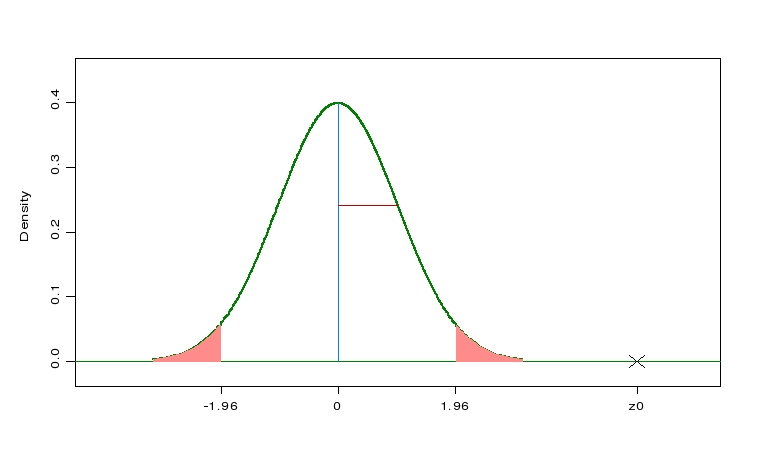
\includegraphics[scale=0.43]{3_16.png}
  \end{figure}
\end{frame}

\begin{frame}
  \vspace*{.25cm}
  \centering
  The null hypothesis $ H_0 $ is accepted\\
  \begin{tiny} (The curve represents the $ Z $ distribution if $ H_0 $ is true) \end{tiny}
  \begin{figure}
    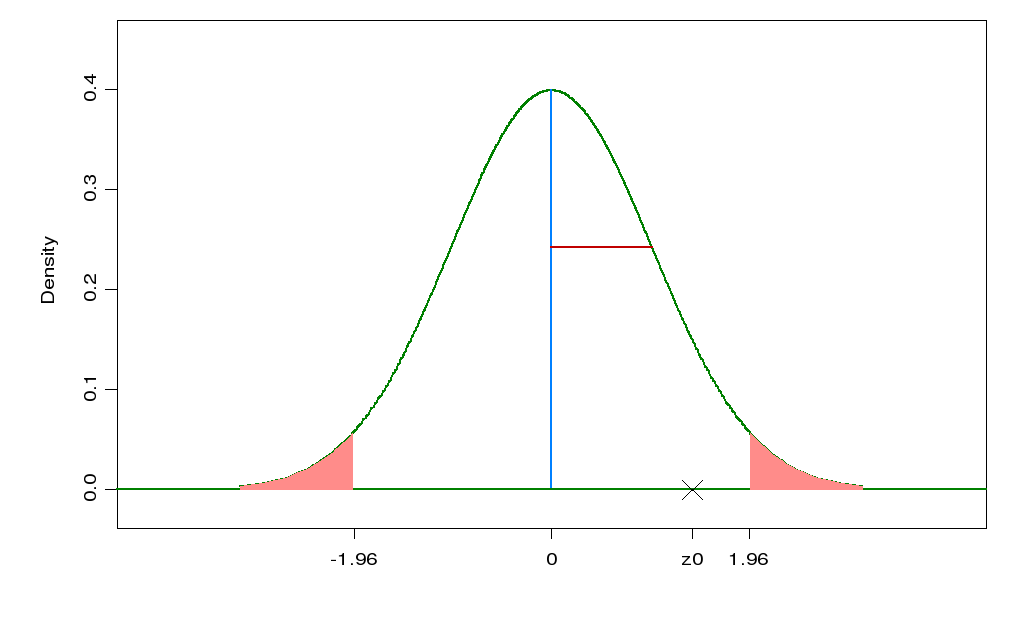
\includegraphics[scale=0.3]{3_17.png}
  \end{figure}
\end{frame}

\begin{frame}
  \vspace*{.25cm}
  \centering
  The null hypothesis  $ H_0 $ is accepted\\
  \begin{tiny} (The curve represents the $ Z' $ distribution, the $ Z $ absolute value, if $ H_0 $ is true) \end{tiny}
  \begin{figure}
    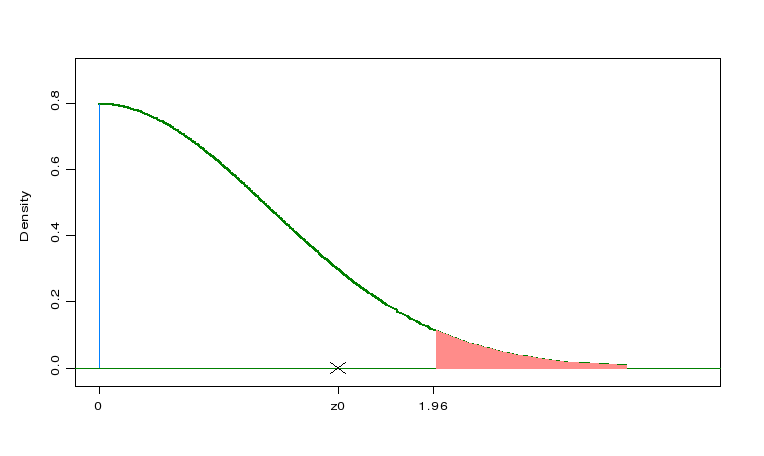
\includegraphics[scale=0.4]{3_18.png}
  \end{figure}
\end{frame}

\begin{frame}
  \begin{small}
    \vspace*{.25cm}
    \textbf{Important notes}.\\
    \vspace*{.25cm}
    The choice of the value 1.96 in the previous formulas is not unjustified, even though it is, in a certain way, arbitrary.\\
    \vspace*{.1cm}
    If the null hypothesis ($ H_0 $) is valid, with the value 1.96, it is possible to have a 0.05 (5$ \% $) probability to commit an error and to refuse this hypothesis.\\
    \vspace*{.2cm}
    This probability is usually shown with the symbol $\alpha$, its corresponding error is called Type I error (or error of the first kind).\\
    \vspace*{.2cm}
    In the statistical hypothesis tests, the Type I error is the only kind of error which is directly verifiable by the reasearcher. Indeed, in the case taken into consideration, when $ \alpha $ increases or decrease, also the ``cut off'' value (1.96) increases or decreases.\\
   \vspace*{.2cm}
   When $ \alpha $ is fixed and, as consequence, the cut-off value is fixed too, the test is called ``of level $\alpha$''.
  \end{small}
\end{frame}

\begin{frame}
  The value 1.96 leaves at its right area a 5$ \% $ probability.\\
  \vspace*{.25cm}
  If the null hypothesis is accepted, or rather if the $ z_0 $ absolute value is at the left of the value 1.96, then the area on the right of the $ z_0 $ absolute value must be greater than 5$ \% $.\\
  \begin{figure}
    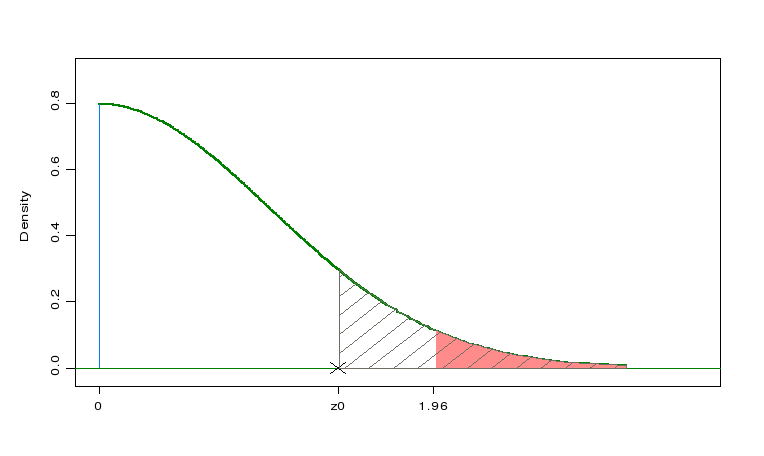
\includegraphics[scale=0.37]{3_20.png}
  \end{figure}
\end{frame}

\begin{frame}
  Thence, another similar criterion to check the null hypothesis consists in measuring the area on the right of the $ z_0 $ value. This measure has to be taken on the distribution that we would have if the null hypothesis is true.\\
  \vspace*{.2cm}
  If $ P \left\{ Z' > z_0 \lvert H_0 \right\} \geq 0.05 $ $\Rightarrow $ we accept $ H_0 $\\
  \vspace*{.1cm}
  If $ P  \left\{ Z' > z_0 \lvert H_0 \right\} < 0.05 $ $\Rightarrow $ we refuse $ H_0 $\\
  \vspace*{.2cm}
  \begin{footnotesize}
    The $ z_0 $ of this formula, that refers to the $ Z' $, distribution, are the $ z_0 $ absolute values (previously seen), referred to the $ Z $ distribution.\\
  \end{footnotesize}
  \vspace*{.5cm}
  The quantity $ P \left\{ Z'>z_0 \lvert H_0 \right\} $ is called \textbf{p-value}.
  This criterion has the advantage of being release from the specific value 1.96. In the same way, it is also release from any other value that isolates, on its right, an area of probability $\alpha$ different from 5$ \% $.
\end{frame}



\livelloA[One or two means inference with Student's t test]{One or two means inference}

\begin{frame}
  \vspace*{.25cm}
  In the experimental  research, the use of an inference test through the sample mean {\boldmath $ \overline{x} $} with {\boldmath $ \sigma $} (the population standard deviation) known  it is a case in a class by itself.\\
  \vspace*{.25cm}
  \textbf{When the population mean {\boldmath $ \mu $} is unknown, also the standard deviation \textbf{\boldmath $ \sigma $}} \textbf{\ is unknown}. As consequence, it is necessary to use a substitute of the variance (the square of the standard deviation) of the population, \textbf{the sample variance {\boldmath $ s^2 $} represents its most logic and most reliable estimation}.\\
  \vspace*{.25cm}
  The statistic test, in this case, is called $ t $, and it is defined as follow:\\
  $$ t = \frac{\overline{x} - \mu_0}{\frac{s}{\sqrt{n}}} $$
\end{frame}

\begin{frame}
  \textbf{With unknown {\boldmath $ \sigma $}} and the use of \textbf{{\boldmath $ s $} as its replacement}, the statistic test prior to sample extraction does not follow the normal distribution $ Z $, previously seen, but the so called \textbf{Student's t} distribution.\\
  \vspace*{.5cm}
  For a better comprehension of the fundamental concepts and a proper application of the derived tests, it is important to highlight the specific characteristics that distinguish this distribution to the Gaussian:\\
  \begin{itemize}
    \item \textbf{the normal distribution considers the {\boldmath $ \overline{X} $} mean sample variation};
    \item \textbf{the Student's t distribution also takes into consideration the sample variability of the standard deviation estimation ({\boldmath $ s $})}.\\
  \end{itemize}
\end{frame}

\begin{frame}
  In order to perform inference on the population mean, starting from sample data, it is necessary to consider at the same time:\\
  \begin{itemize}
    \item \textbf{the variability of {\boldmath $ \overline{x} $} as estimation of {\boldmath $ \mu $}};
    \item \textbf{the variability of {\boldmath $ s $} as estimation of {\boldmath $ \sigma $}}.
  \end{itemize}
  \textbf{With the increase of the sample size {\boldmath $ n $}, {\boldmath $ s $} proves to be an always better estimation of {\boldmath $ \sigma $}.}\\
  \vspace*{.15cm}
  When {\boldmath $ n $} is enough great (in theory infinite, in practice over 120-150), \textbf{{\boldmath $ s $} and {\boldmath $ \sigma $} are almost equivalents}.\\
  \vspace*{.15cm}
  The t-distribution's mean  is 0 (the quantity at the numerator is the difference between the sample mean random variable and its expected value) and the variation that depends on its degrees of freedom (equal to the dimension of the sample minus 1).                                                                                                                                                                                                                                                     
\end{frame}

\begin{frame}
  \vspace*{.25cm}
  As consequence, it could be affirmed that \textbf{when \boldmath{$ n $} increases, the result is the convergence of the Student's \textbf{t} distribution towards the \boldmath{$ Z $}} standard normal distribution.\\
  \vspace*{.25cm}
  With little samples the difference between the Student's \textbf{t} statistics value and the correspondent \boldmath{$ Z $} statistics value at the same probability {\boldmath $ \alpha $} is relevant. On the contrary, over some tens of observations, it is unimportant.\\
  \vspace*{.25cm}
  \textbf{In the experimental practice}, \textbf{the methods which use the t test usually refer to little samples}, the observations are often ten or less and they rarely reach some tens.\\
  \vspace*{.25cm}
  \textbf{The form of the Student's t distribution is symmetric and bell shaped as the normal distribution, but with a larger dispersion (variability)}.
\end{frame}

\begin{frame}
  \vspace*{.5cm}
  \textbf{It exists a whole family of t-distributions, one for each value of the degrees of freedom (df) parameter}.\\
  \vspace*{.5cm}
  For an infinite value of df, in practice for a number of data little greater than an hundred, the {\boldmath $ t $} distribution curve and the {\boldmath $ Z $} distribution curve coincide.\\
  \vspace*{.5cm}
  From the mathematic aspect, this means that \textbf{the normal distribution represents the limit of the {\boldmath $ t $} distribution, when the number of df tends to infinite}.
\end{frame}

\begin{frame}
  \begin{figure}
    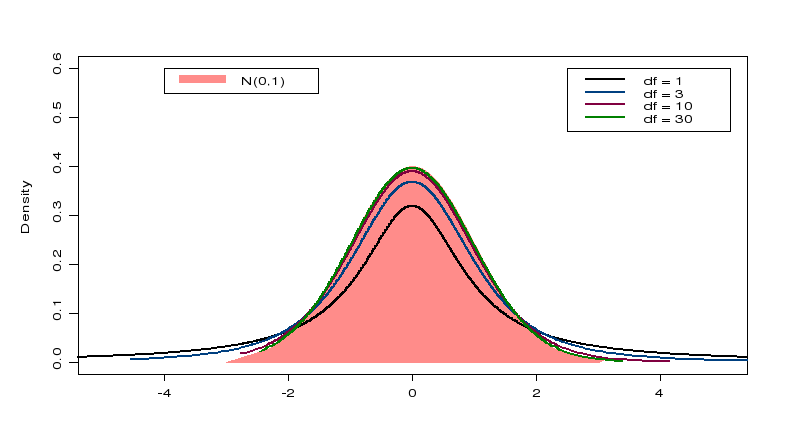
\includegraphics[scale=0.4]{3_27.png}
  \end{figure}
  \hspace*{1cm}Standard normal distribution and Student's t distributions.
\end{frame}

\livelloB[Confidence interval with unknown $\sigma$]{Confidence interval with unknown sigma}

\begin{frame}
  \vspace*{.25cm}
  From the formula $t_{(n-1)}=\frac{\overline{X}-\mu}{\frac{s}{\sqrt{n}}}$, with $\mu$ which, in this case, represents the true and unknown population mean from which the sample is extracted, it is possible to derive the confidence interval at the level  $(1-\alpha)\%$, for the true mean $\mu$, with unknown $\sigma$.\\
  \vspace*{.5cm}
  Once that $\overline{x}$ and $s$, are calculated, the confidence interval with its extremes becomes\\
  $$ \overline{x}- t_{\frac{\alpha}{2};n-1}\cdot \frac{s}{\sqrt{n}} \leq \mu \leq \overline{x}+ t_{\frac{\alpha}{2};n-1}\cdot \frac{s}{\sqrt{n}} $$\\
  where $t_{\frac{\alpha}{2};n-1}$ indicates the t-distribution value with  $ n-1 $ degrees of freedom that ``leaves at its right'' a $\frac{\alpha}{2}$ probability.
\end{frame}

\livelloB{Hypothesis tests}

\begin{frame}
  \vspace*{.25cm}
  \textbf{The applicability conditions to obtain the Student's t distribution}, and therefore, for its use in the tests (we will see them later) and in the confidence intervals are:
  \begin{itemize}
    \item \textbf{the distribution of the single sample units (\textit{X}) is normal};
    \item \textbf{the observations are independently collected}.
  \end{itemize}
  \vspace*{.5cm}
  \textbf{T-tests are robust}. This means that \textbf{their distribution is approximately valid also for data distribution markedly drawn away from the normality.}\\
  This is valid especially if the sample size is large (see Central Limit Theorem).\\
  \vspace*{.25cm}
\end{frame}

\begin{frame}
  \vspace*{-.15cm}
  \begin{figure}
    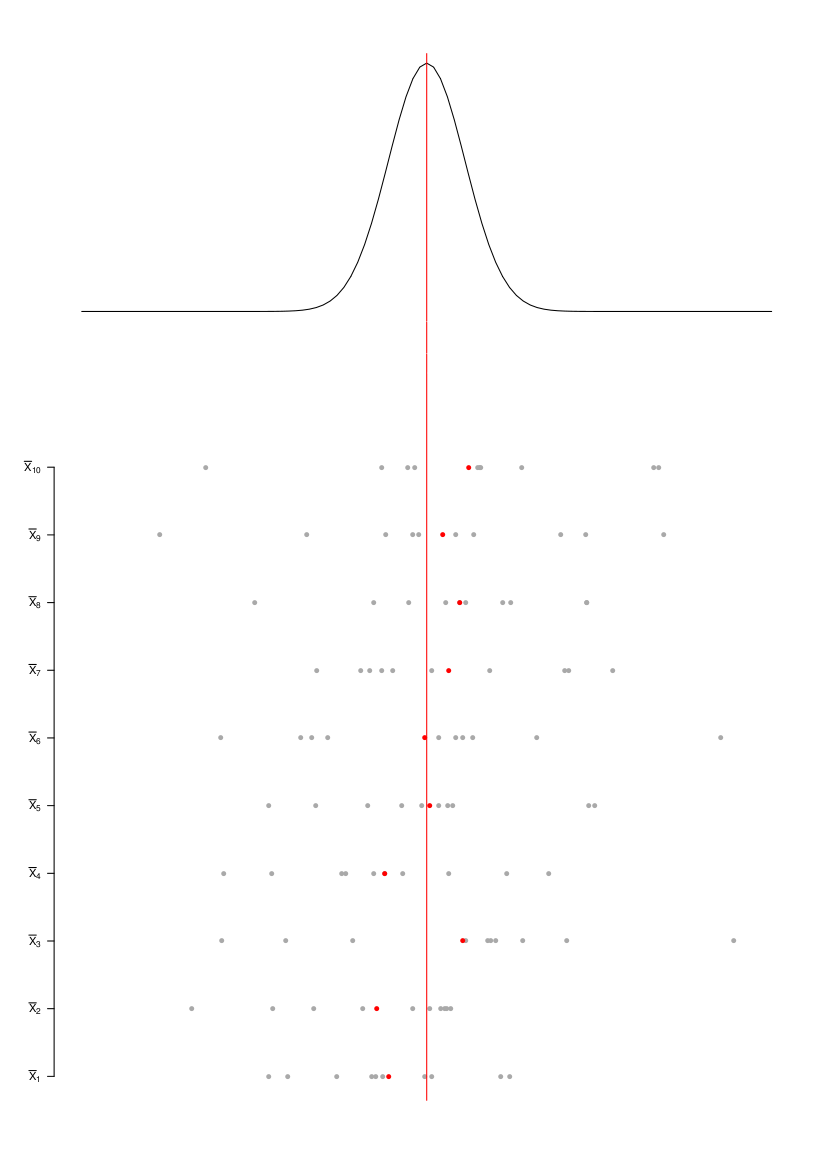
\includegraphics[scale=0.3]{3_tlc.png}
  \end{figure}
\end{frame}

\begin{frame}
  \vspace*{2.5cm}
  \textbf{In general, a test is defined robust as regards the applicability condition, when its results can be accepted even though the applicability condition is not rigorously verified}.
\end{frame}

\begin{frame}
  \vspace*{.5cm}
  In the applied statistics, there are three versions of t-test used to check means:\\
  \vspace*{.25cm}
  \begin{itemize}
    \item \textbf{It checks if the true mean of values of a population is equal to an hypothesize} or expected value (comparison between the observed mean and the hypothesized mean);
    \vspace*{.5cm}
    \item \textbf{It checks if the difference between the true means of values of two independent populations is equal to an hypothesized value} (comparison between independent samples);
    \vspace*{.5cm}
    \item\textbf{It checks if the difference between the true means of values of two dependent populations is equal to an hypothesized value} (comparison between dependent samples).
  \end{itemize}
\end{frame}

\livelloB[Comparison observed mean / hypothesized mean]{Comparison between the observed mean and the hypothesized mean}

\begin{frame}
  \vspace*{.25cm}
  \textbf{In a bilateral test}, in order to specify the hypothesis about the $ \mu $ population mean as regards the expected mean, it will be used the previously seen symbols:
  \vspace*{.25cm}
  \begin{itemize}
    \item \textbf{The null hypothesis} {\boldmath$H_0$} shown as: \hspace*{1.3cm} $H_0: \; \mu \; = \; \mu_0 $\\
    \item \textbf{The alternative hypothesis} {\boldmath$H_A$} shown as: $ H_A: \; \mu \; \ne \; \mu_0$\\
  \end{itemize}
  \vspace*{.25cm}
  Where:\\
  \vspace*{.25cm}
  \begin{itemize}
    \item $ \mu $ is the value (true and unknown) of the population mean from which the sample is extracted and from which will be calculated the sample mean;
    \vspace*{.25cm}
    \item $ \mu_0 $  is the hypothesized value of the mean used as point of mark for the comparison.
  \end{itemize}
\end{frame}

\begin{frame}
  \vspace*{.25cm}
  With the same symbols it is possible to show an unilateral statistical hypothesis test that the population mean, from which the sample is extracted is equal to $\mu_0$ like follows. This is against the alternative that it is smaller than $\mu_0$ will be:
  \begin{itemize}
    \item \textbf{Null hypothesis} {\boldmath $ H_0 $}:  \hspace*{1.45cm} $ H_0: \; \mu \; =\; \mu_0 $\\
    \item \textbf{Alternative hypothesis} {\boldmath $ H_A $}: \hspace*{.15cm} $ H_A: \; \mu \; <\; \mu_0 $\\
  \end{itemize}
  \vspace*{.25cm}
  \textbf{Notes}.
  \begin{itemize}
    \item Unilateralism and bilateralism of a test do not depend on the null hypothesis but on the alternative hypothesis. As a matter of fact, the complete formulation is: test with bilateral and unilateral alternatives.
    \item The difference between the bilateral and unilateral tests is not only applied to t-test but also to Z-test and to all the tests that can make this difference.
  \end{itemize}
\end{frame}

\begin{frame}
  \vspace*{.25cm}
  \textbf{Effectively}.\\
  \vspace*{.5cm}
  After having defined the quantity 
  $$ t=\frac{\overline{X}-\mu_0}{\frac{s}{\sqrt{n}}} $$\\
  Then \textbf{under the hypothesis in which {\boldmath$H_0$} is true}, the $ t $ quantity will be able, prior to extract the sample, to assume a random value that comes from the Student's $ t $ distribution with $ n-1 $ degrees of freedom.\\
  \vspace*{.25cm}
  So, before the experimentation, it is expected that the $ t $ value will be ``concentrated around zero''.\\
\end{frame}

\begin{frame}
  \textbf{In the hypothesis that {\boldmath $ H_0 $} is not true ({\boldmath$H_A$} is true)}, we will have:
  $$ t = \frac{\overline{X}-\mu_0}{\frac{s}{\sqrt{n}}} = \frac{(\overline{X}-\mu)}{\frac{s}{\sqrt{n}}}+\frac{(\mu-\mu_0)}{\frac{s}{\sqrt{n}}}\sim \left[t_{n-1}+\frac{(\mu-\mu_0)}{\frac{s}{\sqrt{n}}}\right] $$
  Before the experimentation, it is expected that the $ t $ value will be approximately far from zero.
\end{frame}

\begin{frame}
  \begin{small}
    The $ t $ value resulting from the experimentation is called $ t_0 $ or rather the $ t $ random variable realization.\\
    According to the formulated alternative hypothesis (unilateral or bilateral), there are two alternatives that respond to the test.\\
    \vspace*{.2cm}
    \textbf{Bilateral hypothesis:}
    \vspace*{-.3cm}
    \begin{itemize}
      \item $ H_0 $ is accepted with an error level of $ \alpha = 0.05 $ when the $ t_0 $ value is between the interval $ \pm t_{n-1;0.025} $. Where $ \pm t_{n-1;0.025} $ is the value of the distribution $ t_{n-1} $ that leaves at its right the 2.5$ \% $ of its overall area.
      \item Alternatively, the null hypothesis is refused in favour of the alternative hypothesis.
    \end{itemize}
    \textbf{Unilateral hypothesis:}
    \vspace*{-.3cm}
    \begin{itemize}
      \item The null hypothesis is accepted with an error level of $ \alpha = 0.05 $ if $ t_0 \geq t_{n-1;(1-0.05)} $ This happens, as in the example, because the alternative hypothesis ($ H_A $) establishes that  $ \mu < \mu_0 $.
      \item Alternatively, if $ t_0 < t_{n-1;(1-0.05)} $, the null hypothesis is refused in favour of the alternative hypothesis.
    \end{itemize}
  \end{small}
\end{frame}

\begin{frame}
  \begin{small}
    \vspace*{.25cm}
    A test \textbf{is unilateral or a one-sided test}, when the researcher asks himself if a mean is larger than the other, excluding that it could be smaller.\\
    \vspace*{.25cm}
    A test \textbf{is bilateral or a two-sided one}, when the researcher asks himself if a significant difference between the two means exists. In this case he does not have information about which one is the larger or the smaller. \\
    \vspace*{.25cm}
    \textbf{In the case of the one-sided test, the refusing area will be in only a part of the distribution (at the left when the sign is negative, at the right when it is positive). In the case of the two-sided test, the refusing area will be symmetrically distributed in the two parts}\\
    \textbf{The probability to demonstrate a significant difference is higher in the case of the one-sided test compared to the two-sided test}. With a technical term \textbf{the two-sided test is more conservative, while the one-sided test is more powerful}.
  \end{small}
\end{frame}

\begin{frame}
  \vspace*{.5cm}
  \begin{figure}
    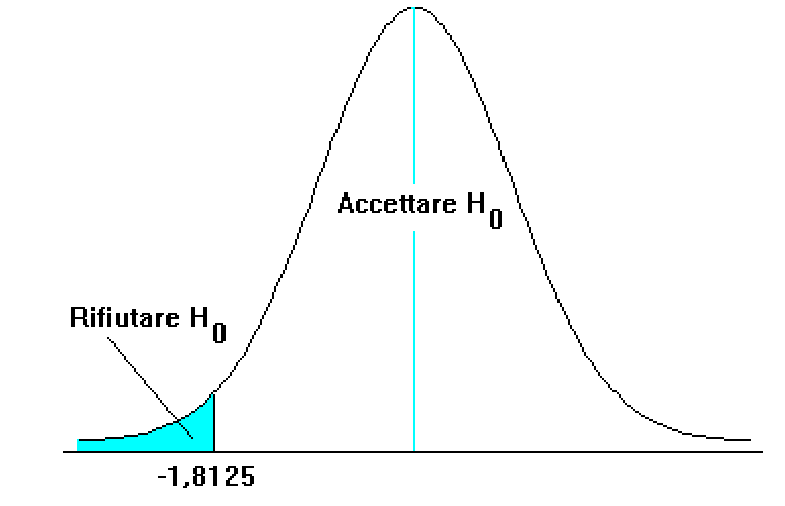
\includegraphics[scale=0.3]{3_38.png}
  \end{figure}
  The unilateral test for a probability associated to a level of statistical significance of 5$ \% $ with 10 df.
\end{frame}

\begin{frame}
  \begin{figure}
    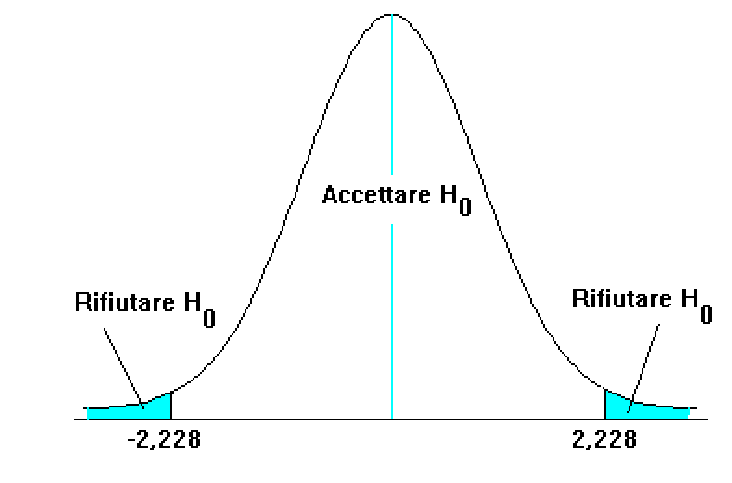
\includegraphics[scale=0.28]{3_39.png}
  \end{figure}
  The bilateral test for a probability associated to a level of statistical significance of 5$ \% $ with 10 df.\\
  \vspace*{.25cm}
  If the test is unilateral it is possible, with the same data, to refuse the null hypothesis. On the contrary, if the test is bilateral, this is not possible.
\end{frame}

\begin{frame}
  \vspace*{.25cm}
  It is possible to use the p-value standard to accept or refuse the null hypothesis both for the $ t $ test and for the $ Z $ test and all the other statistics tests. 
  In this case, the distribution area has to be measured in the case in which the null hypothesis is valid, for values of the statistics tests that go beyond the value that has been found for the same test. For example, with an alternative unilateral hypothesis like $ H_A: \mu < \mu_0 $, and a result $ t_0 $ of the statistics test, then:\\
  \vspace*{.5cm}
  If $ P \left\{ t_{n-1} > t_0 \lvert H_0 \right\} \geq 0.05 $ $ \Rightarrow $ we accept $ H_0 $\\
  \vspace*{.5cm}
  We $ P \left\{ t_{n-1} > t_0 \lvert H_0 \right\} < 0.05 $ $ \Rightarrow $ we refuse $ H_0 $\\
  \vspace*{.5cm}
  If the p-value results to be greater than 0.05, then the null hypothesis is accepted. Otherwise, the null hypothesis is rejected.
\end{frame}

\livelloB{Comparison between means of paired (dependent) samples}

\begin{frame}
  \vspace*{.25cm}
  Student's $ t $ test can be also used to compare the means of two samples. \textbf{The comparison between two means} can be done:
  \begin{itemize}
    \item \textbf{with two dependent samples};
    \item \textbf{with two independent samples}.
  \end{itemize}
  \vspace*{.5cm}
  It is important to distinguish the two situations which depend on the way the two compared measurements are obtained.
  The two tests have differences:
  \begin{itemize}
    \item In the $ t $ test application procedures;
    \item In the way the subjects variability effects are measured.
  \end{itemize}
\end{frame}

\begin{frame}
  \vspace*{.25cm}
  \textbf{The characteristic which distinguishes the comparison between the two dependent samples is to be able to associate each of the samples observations to just one of the observations of the other sample.} The two groups have always, necessarily, the same number of data.\\
  \vspace*{.5cm}
  $ T $ test for two dependent samples is required when the same unities have to be analysed in different conditions.\\
  \vspace*{.25cm}
  For example, to estimate the mean productivity of the staff (in terms of the mean time for each operation) at the beginning and at the end of the working day and to check if this mean changes or not.
\end{frame}

\begin{frame}
  \vspace*{.25cm}
  The comparison between the means of the two series of observations is easy: \textbf{the analysis is applied to a new series of data. This series is the result of the differences between the elements of each couple}.\\
  \vspace*{.5cm}
  For the Student's t test, \textbf{in the case of a bilateral test} the null hypothesis $ H_0 $ is usually that the differences mean is equal to an hypothesize value which is usually 0: \\
  $$ H_0: \; \delta = \delta_0 $$\\
  \vspace*{.25cm}
  \textbf{while the alternative hypothesis} {\boldmath$H_A$} is:\\
  $$ H_A: \; \delta \neq \delta_0 $$
  \vspace*{.25cm}
\end{frame}

\begin{frame}
  \vspace*{.1cm}
  In an \textbf{unilateral test}, \textbf{the null hypothesis} $ H_0 $ is that the differences mean is greater than or equal to the hypothesize one (it is often 0):
  $$ H_0:\;\delta \geq \delta_0 $$
  while \textbf{the alternative hypothesis} $ H_A $ is that the difference is less than the hypothesize one (it is often 0). It can be written like follows:
  $$ H_A:\; \delta < \delta_0 $$
  On the opposite case, \textbf{the null hypothesis} $ H_0 $ is that the differences mean is less than or equal to the hypothesize one (it is often 0):
  $$ H_0:\;\delta \leq \delta_0 $$
  while \textbf{the alternative hypothesis} $ H_A $ is that the difference is greater than the hypothesize one (it is often 0). It can be written like follows:
  $$ H_A:\; \delta > \delta_0 $$
\end{frame}

\begin{frame}
  \vspace*{.25cm}
  In order to choose between the null hypothesis $H_0$ and the alternative hypothesis $H_A$, the statistical significance of the means of the differences is checked by the ratio
  $$t_{(n-1)}=\frac{\overline{d} - \delta_0}{\frac{s_d}{\sqrt{n}}}$$
  where:\\
  \begin{itemize}
    \item $ \overline{d} $ is the mean of the differences;
    \item $ \delta_0 $ is the hypothesize mean difference: it is often, but not necessarily, equal to 0;
    \item $ s_d $ is the standard sample deviation calculated on the differences;
    \item $ n $ is the number of differences. It also corresponds to the number of couples of data (that usually is half of the number of the observations).
  \end{itemize}
\end{frame}

\begin{frame}
  \vspace*{.25cm}
  \textbf{The confidence interval of the differences mean between the two dependent samples is calculated (with the same symbols of the previous formula) by}
  $$ \delta = \overline{d}\pm t_{\frac{\alpha}{2};n-1}\cdot \frac{s_d}{\sqrt{n}}$$\\
  where $t_{\frac{\alpha}{2};n-1}$ indicates the $ t $ distribution value with $ n - 1 $ df that leaves at its right a probability amount equal to $ \alpha/ 2$.\\
  \vspace*{.25cm}
  In this formula it is included, at the level $ 1-\alpha $, the true mean $ \delta $ of the differences.\\
\end{frame}

\begin{frame}
  \vspace*{.25cm}
  \textbf{According to various authors, in the applied field, when the number of couples of data is over 40 (others indicates 50 or even 150), the Student's $ t $ distribution is adequately approximated to the standard normal distribution}.\\
  \vspace*{.5cm}
  \textbf{In the variance calculation formula}, with a difference in the results that a great number of researchers consider unimportant, \textbf{when the dimension of {\boldmath$ n $} measures some tens, it is possible to replace the critic {\boldmath$ t $} value with the {\boldmath$ Z $} value associated to the prefixed probability   {\boldmath$\alpha$}. This situation happens both in the one-sided tests and in the two-sided tests}.
\end{frame}

\livelloB{Comparison between means of independent samples}

\begin{frame}
  \vspace*{.25cm}
  In a great amount of cases, it is not possible and even plausible to get two dependent samples.\\
  The only possible strategy  for the analysis of data is \textbf{to compare two independent samples and two samples formed by different individuals}.\\
  \vspace*{.5cm}
  In this case \textbf{the result is the increase of the variability within the two groups} but it is also possible to obtain three advantages:
  \begin{itemize}
    \item \textbf{a different number of observations in the two groups can be used};
   \item \textbf{to have data that are easier the expression of the random variability};
   \item \textbf{to be able to use samples taken from different units for the comparison}.
\end{itemize}
\end{frame}

\begin{frame}
  \vspace*{.25cm}
  With the statistical significance test for two independent samples, it is checked \textbf{the same hypothesis of the case of paired data, even though it is expressed in a different way}.\\
  \vspace*{.25cm}
  It is fundamental to understand that:\\
  \begin{itemize}
    \item for two dependent samples, the calculation are done just on the differences; 
    \item in the case of two independent samples \textbf{the calculation are done on the two series of observations}.
  \end{itemize}
  \vspace*{.25cm}
  In a  \textbf{bilateral or a two-sided test}, \textbf{the null hypothesis} $ H_0 $ is that the difference between the two populations (A and B) is equal to $ \delta_0 $. Quite always $ \delta_0 $ is equal to 0 in the practice use.
\end{frame}

\begin{frame}
  \vspace*{.25cm}
  The null hypothesis can be written as:
  $$ H_0: \; \mu_A \; - \; \mu_B \; = \delta_0 \mbox {\hspace*{.5cm}or\hspace*{.5cm}} \; H_0: \; \mu_A \; = \delta_0 + \mu_B \; $$
  and its \textbf{bilateral alternative hypothesis } $ H_A $ can be written as:\\
  $$ H_A: \; \mu_A \; - \; \mu_B \; \neq \delta_0 \mbox{\hspace*{.5cm}or\hspace*{.5cm}} \; H_A: \; \mu_A\; \neq \delta_0 +\mu_B \; $$ \\
  \vspace*{.5cm}
  An example \textbf{of  one-sided or unilateral test} is:
  $$ H_0: \; \mu_A \; - \; \mu_B \; \leq \delta_0 \mbox{\hspace*{.5cm}or\hspace*{.5cm}} \; H_0: \; \mu_A \; \leq \delta_0 + \mu_B \; $$ \\
  \vspace*{.25cm}
  against the alternative hypothesis:
  $$ H_A: \; \mu_A \; - \; \mu_B \; > \delta_0 \mbox{\hspace*{.5cm}or\hspace*{.5cm}} \; H_A: \; \mu_A \; > \delta + \mu_B\; $$
\end{frame}

\begin{frame}
  \begin{small}
    \vspace*{.25cm}
    In the case of two independent samples, in its easier formulation, the value of $ t $ is obtain like follows:
    $$ t_{(n_A+n_B-2)} = \frac{(\overline{X}_A-\overline{X}_B)-\delta_0}{\sqrt{S^2_p \cdot (\frac{1}{n_A}+\frac{1}{n_B})}} $$ \\
    \vspace*{.25cm}
    And the degrees of freedom of $ t $  are equal to $ (n_A-1)+(n_B-1)=(n_A+n_B-2)$, or $(N-2) $.\\
    \vspace*{.15cm}
    \begin{itemize}
      \item $ \overline{X}_A $ and $ \overline{X}_B $ are the means calculated respectively on the (sub) sample A and on the (sub) sample B;
      \item $ \delta_0 = (\mu_A - \mu_B) $ is the hypothesized difference between the means. It is expressed in the null hypothesis;
      \item $ n_A $ and $ n_B $ are the number of observation in the (sub) samples A and B;
      \item $ N = n_A + n_B $;
      \item $ S^2_p $ is the (\textit{pooled}) variance of the compared groups.
   \end{itemize}
  \end{small}
\end{frame}

\begin{frame}
  \begin{small}
%     \vspace*{.25cm}
    \textbf{The pooled variance} ({\boldmath$ S^2_p $}) is the result of the ratio between the sum of the two deviances and the sum of the respective df:\\
    \vspace*{.25cm}
    $$ S^2_p = \frac{\sum_{i=1}^{n_A}{(X_{A_i}-\overline{X}_A)^2}+\sum_{i=1}^{n_B}{(X_{B_i}-\overline{X}_B)^2}}{n_A-1+n_B-1} $$\\
    \vspace*{.25cm}
    where:
    \begin{itemize}
      \item $ X_{A_i} $ and $ \overline{X}_A $ are respectively the data and the sample mean of the group \textbf{A};
      \item $ X_{B_i} $ and $ \overline{X}_B $ are respectively the data and the sample mean of the group \textbf{B};
      \item $ n_A $ and $ n_B $ are the number of observation of samples \textbf{A} and \textbf{B}.
    \end{itemize}
    \vspace*{.25cm}
    The pooled variance \textbf{is a weighted average variance, calculated starting from the two deviances and from their df}. The pooled variance assigns a proportionally higher importance to the group which has a greater number of data.
  \end{small}
\end{frame}

\begin{frame}
  \vspace*{.25cm}
  $$ t_{(n_A+n_B-2)} = \frac{(\overline{X}_A-\overline{X}_B)-\delta}{\sqrt{S^2_p \cdot (\frac{1}{n_A}+\frac{1}{n_B})}} $$\\
  \vspace*{.25cm}
  From the above t test formula it is possible to deduce that, in order to calculate the test it is not necessary that all the data (of the extracted selection unities) are available.\\
  \vspace*{.5cm}
  The formula can be calculated starting from the means, the standard deviations and the sample size of the two samples.
\end{frame}



\livelloA{Testing the equality of two variances}

\begin{frame}
  \vspace*{.25cm}
   \textbf{The Student's t test} (in the form we have just seen) is a \textbf{parametric statistics test}. In other words, it is based on the characteristics of the \textbf{normal distribution} which is defined by \textbf{parameters} like the \textbf{mean} and the \textbf{variance}, the \textbf{symmetry} and the \textbf{kurtosis}. The application of this test, in order to be considered valid, \textbf{required the three following conditions}:
  \vspace*{.35cm}
  \begin{itemize}
    \item  \textbf{the independence of the data within and between the samples};
    \vspace*{.25cm}
    \item  \textbf{the homogeneity of the variances} (the comparison between two or more means is valid \textbf{only if} the samples extracted from the populations have a similar variance);
    \vspace*{.25cm}
    \item \textbf{the data (or the residual compared to the mean) are normally distributed}.
  \end{itemize}
\end{frame}

\begin{frame}
  \vspace*{.25cm}
  Whit \textbf{two independent samples}, the most important applicability condition is the variances uniformity because, compared to it, the \textbf{$ t $ test is less robust}.\\
  \vspace*{.25cm}
  In order to  \textbf{calculate the \boldmath$ S^2 $ pooled}, it is necessary that condition of \textbf{homoscedastic} is realised. This means that \textbf{the two variances should be statistically equal}.\\
  \vspace*{.25cm}
  The hypothesis of independent collection of data depends on the plan  of the experimentation. The hypothesis of normality of the data or of the error (the data residuals from their mean) can be violated without serious effects on the power and on the result of the test; this happens unless there is a serious asymmetry but \textbf{the equality of the two independent samples variance should be always checked}.
\end{frame}

\begin{frame}
  \vspace*{.25cm}
  From the intuitive point of view, this concept can be easily explained. The variance can be considered as a reliability estimation of a mean that represents the population.\\
  \vspace*{.25cm}
  The data that are really variable (with a wide variance) have less reliable means for the same number of observations. This happens because they are more variable, as their data. To compare the two means it is necessary that their reliability is similar.\\
  \vspace*{.25cm}
  For the application of the t-test, the homoscedastic between two groups (\textbf{A} and \textbf{B}) is checked with a \textbf{bilateral test}, where the null hypothesis $ H_0 $ and the alternative hypothesis $ H_A $ are:
  $$ H_0: \, \sigma^2_A = \sigma^2_B \mbox{\hspace*{2cm}} H_A: \, \sigma^2_A \neq \sigma^2_B $$
\end{frame}

\begin{frame}
  \vspace*{.25cm}
  \textbf{The most popular tests} to check the homoscedastic are three:
  \vspace{.25cm}
  \begin{itemize}
    \item the \textbf{F-test} or the ratio between the two variance;
    \vspace*{.25cm}
    \item the \textbf{Levene's test};
    \vspace*{.25cm}
    \item the \textbf{Bartlett's test}.
  \end{itemize}
  \vspace*{.5cm}
  It should be possible to use \textbf{Student's t test for two independent samples} only if \textbf{it is demonstrated that the null hypothesis is true} and therefore that the two groups have statistically equal variances.
\end{frame}

\livelloB{F test of equality of variances}

\begin{frame}
  \vspace*{.25cm}
  The \textbf{bilateral F-test}, is the most difficult and the first that has been purposed. It is founded on the \textbf{ratio between the larger sample variance ({\boldmath $ s^2 $}) and the smaller sample variance}:\\
  \vspace*{.25cm}
  $$ F_{(n_1-1);(n_2-1)} = \frac{S^2_1}{S^2_2} $$\\
  \vspace*{.25cm}
  where:
  \vspace*{.25cm}
  \begin{itemize}
    \item $ S^2_1 $ is the larger variance;
    \item $ S^2_2 $ is the smaller variance;
    \item $ n_1 $ is the number of observations in the group with the larger variance;
    \item $ n_2 $ is the number of observations in the group with the smaller variance.
  \end{itemize}
\end{frame}

\begin{frame}
  \vspace*{.25cm}
  Under the hypothesis in which the two variances are equal (the null hypothesis $H_0$ is true), the result of the ratio between them should be close to 1. It is obviously admitted a certain tolerance, because the estimation of the two samples variances is never exact.\\
  \vspace*{.25cm}
  In the practice, the variances are often estimated on small samples, formed by few units of observations. As consequence, the ratio between the two variances is a sample estimation, that could vary from \textbf{one to infinite} or \textbf{from one to zero}.\\
  \vspace*{.25cm}
  In order not to use both the measures, which will give a redundant information, it has been chosen the values distribution which is more sensitive to the variations: that from one to infinite.
\end{frame}

\begin{frame}
  \vspace*{.25cm}
  If the hypothesis $ H_0 $ is valid, then the quantity $ F_{(n_1-1);(n_2-1)} $ will be a F of Fisher-Snedecor random variable with $ (n_1-1),\,(n_2-1) $ degrees of freedom. It will tend to concentrate most part of its distribution around 1.\\
  \vspace*{.25cm}
  If, on the contrary, the hypothesis $ H_A $ is valid, then $ F_{(n_1-1);(n_2-1)} $ tends to have greater values than the expectation.\\
  \vspace*{.25cm}
  It will be necessary, then, to check with which probability a F random variable tends to have values equal or greater than the one obtained by the samples data. If this probability is little (this means, less than $ \alpha $), then the null hypothesis $ H_0 $ is rejected in favour of the alternative one. 
  Otherwise, the null hypothesis that the two variances are not statistically different, is accepted.
\end{frame}

\livelloB{Levene's test}

\begin{frame}
  \vspace*{.25cm}
  The \textbf{Levene's Test} is an \textbf{alternative method}. It can be used also to integrate the analysis that has been done with the F-test when a more thorough valuation on the two variances homogeneity wants to be found.\\
  \vspace*{.25cm}
  Levene's test is considered from certain statisticians \textbf{more robust than F-test} as regards the non-normality of the distribution. It is mainly spread because of its introduction in certain statistical tools.\\
  \vspace*{.25cm}
  This test compares the residuals either from the means or from the medians of the two groups i.e. the differences ($ d_i $) compared to the means (or medians) of the groups:
  $$ d_i = X_i-\overline{X} $$
\end{frame}

\begin{frame}
  \vspace*{.25cm}
  after\\
  \begin{itemize}
    \item having taken the square root
    $$ d_i = (X_i - \overline{X})^2 $$
    \item or taking them in absolute value
    $$ d_i = \abs{X_i - \overline{X}} $$
  \end{itemize}
  \vspace*{.25cm}
  in order to \textbf{eliminate the negative signs}.\\
  \vspace*{.25cm}
  The two methods provide \textbf{different results}: the variance is larger and then the power is smaller with the use of the square of the residuals.
\end{frame}

\begin{frame}
  \vspace*{.25cm}
  The second method, that uses the residual in absolute value \textbf{is the most used one} mainly in the computer programs. It has similar tests in the non-parametric statistics.\\
  \vspace*{.5cm}
  In order to compare the variance of the two groups (\textbf{A} and \textbf{B}),\\
  \vspace*{.25cm}
  with null hypothesis
  $$ H_0: \, \sigma^2_A = \sigma^2_B $$\\
  \vspace*{.5cm}
  and with bilateral alternative hypothesis
  $$ H_A: \, \sigma^2_A \neq \sigma^2_B $$
\end{frame}

\begin{frame}
  \vspace*{.25cm}
  \textbf{Levene's propose consists in the application of the Student's t test to the two series of residuals} (in square or in absolute value). It assumes that, \textbf{ if their means values are significantly different, the two variances of the original data are different too}.\\
  \vspace*{.5cm}
  If, \textbf{by the use of the residuals mean}, the null hypothesis is refused
  $$ H_0: \, \mu^2_A = \mu^2_B $$\\
  \vspace*{.25cm}
  in order to accept the alternative hypothesis
  $$ H_A: \, \mu^2_A \neq \mu^2_B $$
  (where the $ \mu^2_K $ in this case, represent the means residuals in square or in absolute value in the two groups).
\end{frame}

\begin{frame}
  \vspace*{.25cm}
  implicitly it comes that:\\
  \vspace*{.5cm}
  on \textbf{the original datai} the null hypothesis is refused \hspace*{1.3cm} $ H_0: \, \sigma^2_A = \sigma^2_B $ \\
  \vspace*{.5cm}
  in favour of the alternative hypothesis \hspace*{2.6cm} $ H_A: \, \sigma^2_A \neq \sigma^2_B $\\
  \vspace*{1cm}
  Also \textbf{Levene's test can be useful to check the unilateral hypothesis}\\
  \vspace*{.25cm}
  the null hypothesis \hspace*{5.5cm} $ H_0: \, \sigma^2_A \geq \sigma^2_B $ \\	
  \vspace*{.5cm}
  against the alternative hypothesis \hspace*{3.4cm} $ H_A: \, \sigma^2_A < \sigma^2_B $\\
\end{frame}

\livelloB{Bartlett's test}

\begin{frame}
  \vspace*{.25cm}
  \textbf{In order to make the Bartlett's test, it is enough to apply the unilateral t-test to the residuals means}.\\
  \vspace*{1.25cm}
  \textbf{Bartlett's test} uses the $\chi^2$ distribution.\\
  \vspace*{.25cm}
  In order to check the hypothesis of homoscedastic between the two independent samples, the synoptic table of $ \chi^2_{(1)} $ \textbf{with one degrees of freedom is used}. 
\end{frame}

\begin{frame}
  \begin{small}
    \vspace*{.25cm}
    It is \textbf{important} to remember that it is necessary to act cautiously in the use of the inference for the homoscedastic. As consequence, this is also valid to conclude that two variances are similar and to apply Student's t test on the means.\\
    \textbf{Statistics tests are generally structured not to refuse the null hypothesis}, unless there is evidence of the contrary: \textbf{The null hypothesis is refused only when it is proved that there is a little probability to find, by coincidence, differences as large as the found one, or larger}.\\
    \vspace*{.25cm}
    In order to have a significant test, if the researcher has few data, the differences between the two groups have to be really large: \textbf{A test with few data is not very powerful. This means that it has few possibilities to refuse the null hypothesis, even when it is known that it is false}.\\
    \vspace*{.25cm}
    As consequence, mainly in these cases, \textbf{ when the null hypothesis {\boldmath $ H_0 $} is not refused, it is not possible to affirm that it is true}. It is only impossible to affirm that it is false because of the few information.
  \end{small}
\end{frame}

\begin{frame}
  \begin{small}
    \vspace*{.25cm}
    In operational terms it is possible to go out from this illogical use of the tests for homoscedastic thanks to  \textbf{a more complete and detailed valuation of the estimated probability {\boldmath $ \alpha $}}.\\
    With few data, if the probability $ \alpha $ is little higher than 0.05 (for example 0.10 or 0.15) it is not possible to refuse the null hypothesis. If it would have been possible to have a greater number of data, with an high probability, it would have been possible to refuse the null hypothesis.\\
    \vspace*{.25cm}
    In practice, according to certain authors, it would be better to accept the null hypothesis only when the calculated probability $ \alpha $ is high, higher than 30\%. With a greater number of data, this probability can be lowered to 20\%. Unfortunately, it does not exist specific rules to define a large or small sample and to decide to which level of probability $ \alpha $ it is possible to affirm that the null hypothesis is true. The choice is based on the statistical common sense, that can only come from the experience.
  \end{small}
\end{frame}



\livelloA{Testing the normality}

\begin{frame}
  \vspace*{.25cm}
  The tests that have been analysed so far are based on the conditions of normality of data (even though, sometimes, not in a ``strong'' way because of the robustness of the \textit{t} test to the deviation of the conditions of normality).\\
  \vspace*{.25cm}
  Anyway, in the real world, the natural phenomenon does not always (sometimes rarely) behave like Gaussian random variables.\\
  \vspace*{.25cm}
  It is obvious that a certain argument cannot be taken for granted and has to be, on the contrary, checked on the data.\\
  \vspace*{.25cm}
  With this aim, different statistics tests have been produced. Some of them are the numerical type and others the graphic type.
\end{frame}

\begin{frame}
  \vspace*{.25cm}
  Some of the most known numerical tests of normality are:
  \begin{itemize}
    \item Kolmogorov-Smirnov test
    \item Kolmogorov-Smirnov test with Lilliefors' tabulated probability
    \item Shapiro-Wilk W test
    \item Anderson-Darling test
  \end{itemize}
  \vspace*{.25cm}
  The most known graphic test to check the normality is the \textit{Normal Probability Plot}.\\
  \vspace*{.25cm}
  Anderson-Darling test and the \textit{Normal Probability Plot} are afterwards described. 
\end{frame}

\livelloB{Anderson-Darling's test}

\begin{frame}
  \vspace*{.25cm}
  The following plot represents the cumulative histograms of two distributions (one normal and the other not normal) with the normal cumulative distribution (estimated) written above.
  \begin{figure}
    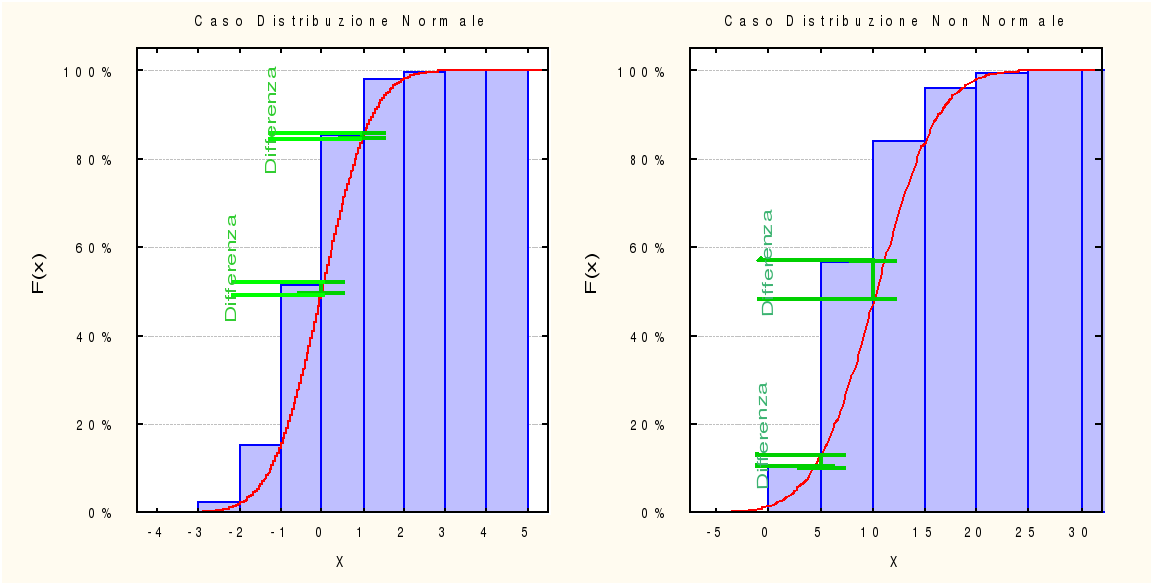
\includegraphics[scale=0.27]{3_81.png}
  \end{figure}
\end{frame}

\begin{frame}
  \begin{small}
    \vspace*{.25cm}
    The Anderson-Darling test calculates the square mean difference between the ``true'' cumulative distribution (the one obtained by the observed data) and the theoretic (obtained by the hypothesis in which the data are distributed as a Gaussian). The approximation of this difference is calculated by the following formula:\\
    \vspace*{.25cm}
    $$ AD = \sum_{i=1}^n {\frac{1-2i}{n}}\{\ln(F_0[Z_{(i)}])+\ln(1-F_0[Z_{(n+1-i)}])\} - n $$\\
    \vspace*{.25cm}
    where $ n $ is the sample dimension, $ Z_{(i)} $ are the orderly and standardized values that has been observed, $ F_0 $ is the cumulative distribution of the standard Gaussian.\\
  \vspace*{.25cm}
  In the hypothesis in which data are effectively generated by a Gaussian (the picture on the left), it is expected a little mean quadratic difference.\\
  In the hypothesis in which the data are generated by a different distribution from the Gaussian, it is expected a large mean quadratic difference.                                                                                                                                               \end{small}
\end{frame}

\begin{frame}
  \vspace*{.25cm}
  The p-level (or the rejection cut-off value) depends on the analysed distribution and it is not a simple calculation.\\
  \vspace*{.75cm}
  When the normality is checked, the AD value for which rejecting the null hypothesis, at the level $ \alpha=0.05 $ is given by the formula:\\
  \vspace*{.5cm}
  $$ AD > \frac{0.752}{(1 + \frac{0.75}{n} + \frac{2.25}{n^2})} $$
\end{frame}

\livelloB{The normal probability plot}

\begin{frame}
  \vspace*{.25cm}
  The \textbf{normal probability plot} is a graphic tool. It is useful to evaluate the normality of the distribution of a sample of observed data.\\
  \vspace*{.35cm}
  It is supposed to have a sample of $ n $ independent observations: $ x_1, \; x_2, \; \dots, \; x_n $ come from the same unknown distribution\\
  \vspace*{.35cm}
  The data are arranged according to their value, in an ascending order. In this way an ordered sample is obtained: $ x_{(1)}, \; x_{(2)}, \; \dots, \; x_{(n)} $.\\
  \vspace*{.35cm}
  The $ i $th observation of the ordered sample will correspond to the $ i $th  observed quantiles. Furthermore, it will be a reasonable estimation of the $ i $th quantiles of the distribution (true and unknown) from which the data come.
\end{frame}

\begin{frame}
%   \vspace*{.25cm}
  The idea that stands at the basis of the normal probability plot is to compare the estimated percentiles values with the values of the correspondent theoretic percentiles that come from the standard normal distribution.\\
  \vspace*{.25cm}
  \textbf{Example}.\\
  It is supposed to have ten observations (already ordered):\\
  \begin{tabular}{llllllllll}
    0.73 & 1.34 & 1.44 & 1.68 & 1.77 & 1.78 & 1.95 & 2.4 & 2.95 & 3.93
  \end{tabular}\\
  The first observation is the estimation of the first deciles (quantiles 1/10) for the data origin distribution. The value of the correspondent quantiles for the standard normal distribution is more or less -1.28.\\
  The second observation is the estimation of the second deciles (quantiles 2/10) for the data origin distribution. The value of the correspondent quantiles for the standard normal distribution is more or less -0.84.\\
  The third observation is the estimation of the third deciles, and so on.
\end{frame}

\begin{frame}
  \vspace*{.25cm}
  The result of the elaboration of the data is a table with $ n = 10 $ couples of values. If these couples are drawn in a scatter plot, the result is the following plot:
  \begin{figure}
    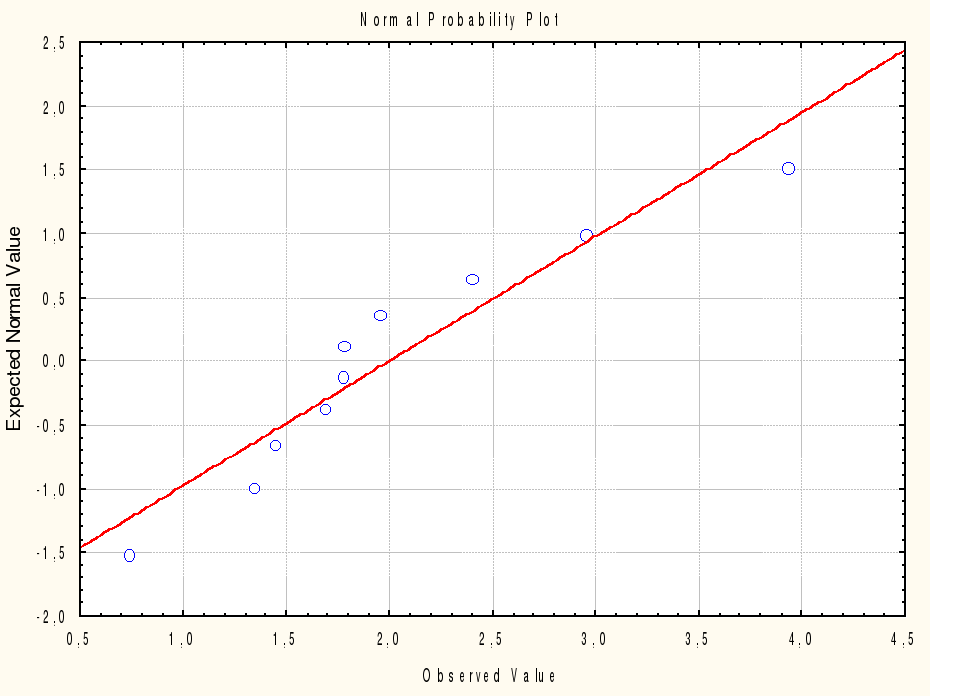
\includegraphics[scale=0.17]{3_86.png}
  \end{figure}
  If the points tend to place around a line, then it is possible to accept the hypothesis that the origin distribution of our data is normal.
\end{frame}

\begin{frame}
  \begin{small}
%     \vspace*{.25cm}
    \textbf{Some notes}.
    \begin{itemize}
      \item The line that has been drawn in the previous plot is usually added in order to facilitate the reading of the ``linearity'' of the points disposition. Particular meanings of the slope or of the intercept of this line do not have to be searched.
      \item The percentiles estimation usually follows some rules a little bit more complex than the previous one. As a result, it will be obtained more considerable estimations. Anyway, the logic of the plot creation is the one we talked about.
      \item  In the normal probability plot the data in the tails of the plot are usually less reliable. This happens mainly when there is a small sample size.
      \item The previous plot is concerning a sample that comes from the normal distribution. Take in consideration the sample size!
      \item Afterwards, some examples of normal probability plot for large samples that come from different distribution will be explained.
    \end{itemize}
  \end{small}
\end{frame}

\begin{frame}
  \vspace*{.25cm}
  \begin{figure}
    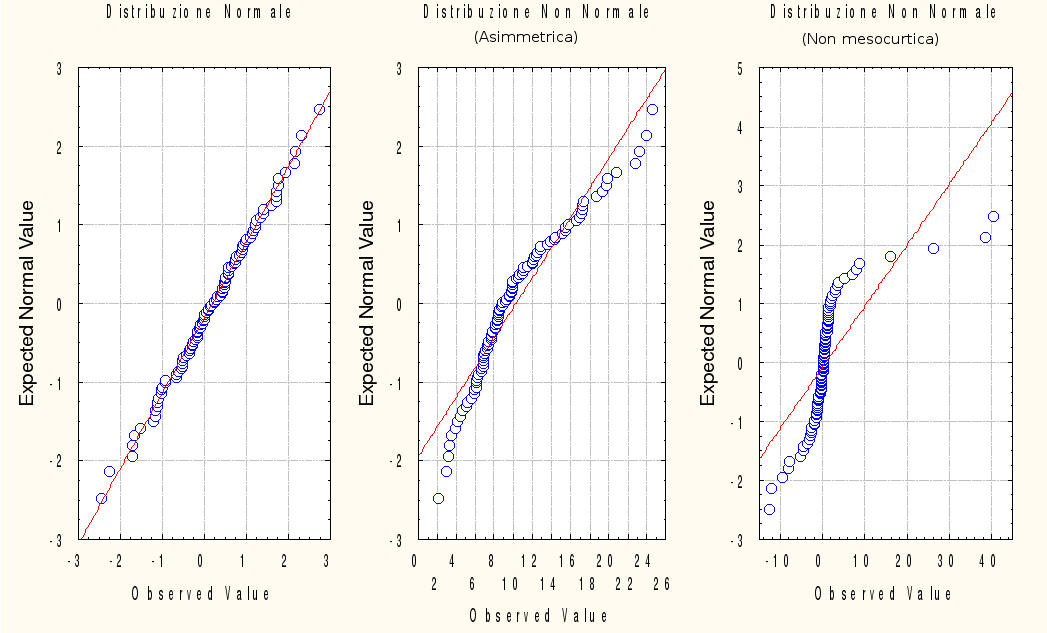
\includegraphics[scale=0.3]{3_88.png}
  \end{figure}
\end{frame}



\livelloA{Proportion tests}

\livelloB{One proportion p test}

\begin{frame}
  \vspace*{.75cm}
  For qualitative type phenomenon, the interest is often in the (percentage) ratio of units which present the interesting characteristic.\\
  \vspace*{.5cm}
  For exampleit can be useful to know: in the case of a productive process, the percentage of the defective pieces; in a clinical reasearch, the proportion of people who positively respond to a medicine; in a bank, the proportion of insolvent customers.\\
  \vspace*{.5cm}
  All of these phenomenon can be modeled with a binomial random variable of parameters $ n $ and $ p $. $ n $ indicates the number of proofs (trials) and $ p $ indicates the probability of success in every single trial, which is supposed to be equal in each trial.\\
\end{frame}

\begin{frame}
  It wants to be checked the hypothesis that the true (and unknown) proportion of interest events (happened) is $ p_0 $ starting from sample data. This is against the alternative hypothesis which is different.\\
  \begin{tabbing}
    The null hypothesis is formulated: \=  $ H_0 $ \= $ :  p = p_0 $,\\
    Against the alternative hypothesis: \>  $ H_A $ \> $ :  p \neq p_0 $.\\
  \end{tabbing}
  \vspace{-0.5cm} 
  $ {x} $ is the number of ``successes'' obtained after having done $ n $ trials. $ \hat{p} = \frac{x}{n} $ is the proportion of ``successes'' in the sample.\\
  In its easiest formulation, the p-test for a proportion is like follows:
  $$ \frac{\hat{p} - p_0}{\sqrt{p_0 (1-p_0) / n}} $$
  That, if $ H_0 $  is valid and $ n $ is enough large, it is distributed like a normal standard.
\end{frame}

\begin{frame}
  \vspace*{.25cm}
  \textbf{Example}.\\
  \vspace{0.25cm}
  A factory that produce DVDs wants to check the hypothesis that the proportion of defective pieces is 0.01 (=1$ \% $), to a level of statistical significance $ \alpha = 0.05 $.\\
  \vspace{0.25cm}
  With this aim, it selects, by chance, 100 pieces and it tests them. The result of the test shows that there are always two defective pieces.\\
  \vspace{0.25cm}
  In order to check the null hypothesis $ H_0: p = 0.01 $ against the alternative hypothesis $ H_A: p \neq 0.01 $, it is necessary to use the previously seen statistics:
  $$ \frac{(2/100) - 0.01}{\sqrt{0.01 (1-0.01) / 100}} = 0.01 / \sqrt{0.000099} = 1.005 $$\
\end{frame}

\begin{frame}
  \vspace{0.25cm}
  It is possible to conclude that \textbf{ it does not exist empirical evidence that allows to refuse the null hypothesis}. This conclusion is obtained because the obtained quantity (1.005), in absolute value, is smaller than the cut-off value of a normal standard for $ \alpha = 0.05 $, which is 1.96.\\ 
  \vspace{0.5cm}
  It is possible to reach the same conclusion observing the p-value, that can be calculated as the probability to have, in a standard normal distribution, a value smaller than -1.005 or the probability to have a greater than 1.005 one. This probability is 0.315. Since the p-value is greater than the fixed $ \alpha $ value, the null hypothesis is not refused.
\end{frame}

\begin{frame}
  \vspace{0.25cm}
  It is possible to build a confidence interval for the ``true'' proportion of successes. This is, similarly to what has been seen for the Z-test, the interval:
  $$ \left( \hat{p} - z_{1-\frac{\alpha}{2}} \cdot \sqrt{\frac{p_0 (1-p_0)}{n}}; \hat{p} + z_{1-\frac{\alpha}{2}} \cdot \sqrt{\frac{p_0 (1-p_0)}{n}} \right) $$\\
  \vspace{0.25cm}
  \textbf{Example}.\\
  The true proportion of defective DVDs at a confidence level of $ 0.95 $, with the data we have seen in the previous example, is:
  $$ \left( \frac{2}{100} - 1.96 \cdot \sqrt{\frac{0.01 (1-0.01)}{100}}; \frac{2}{100} + 1.96 \cdot \sqrt{\frac{0.01 (1-0.01)}{100}} \right) $$
  That is the interval $ \left(0.0005; 0.0395\right) $.
\end{frame}

\begin{frame}
  \vspace{0.5cm}
  As regards both the statistical hypothesis test and the building of the confidence intervals, various methodologies exist. Those that have been already shown, are the easiest versions.\\
  \vspace{0.5cm}
  As regards the statistical hypothesis tests, it also exists an exact version of the test, based on the Beta distribution.
\end{frame}

\livelloB{Two proportions p test}

\begin{frame}
  In the case of two means coming from different samples, it has been seen how it is possible to check the hypothesis that the two populations true (and unknown) means, are equal. In the same way, in the case of two samples, it is possible to check, starting from sample data, the hypothesis that the true proportions ($ p_A $ and $ p_B $) of two different populations are equal.\\
  \vspace{-.5cm}
  \begin{tabbing}
    The null hypothesis is formulated: \=  $ H_0 $ \= $ :  p_A = p_B $,\\
    Against the alternative hypothesis: \>  $ H_A $ \> $ :  p_A \neq p_B $.\\
  \end{tabbing}
  \vspace{-.5cm}
  In its easiest formulation, the p-test for two proportions has the following form:
  $$ \frac{\hat{p}_A - \hat{p}_B}{\sqrt{\hat{p}_A (1 - \hat{p}_A) / n_A + \hat{p}_B (1 - \hat{p}_B) / n_B}} $$
  That, if $ H_0 $ is true and with $ n_A $ and $ n_B $ enough large, it is distributed as normal standard.
\end{frame}

\begin{frame}
  \vspace{0.25cm}
  \textbf{Example}.\\
  It is supposed that two different machineries, A and B, have produced respectively 200 and 500 pieces within a working day. 3 of the pieces produced by the machinery A and 4 of the pieces produced by the machinery B were defective.\\
  \vspace{0.25cm}
  It wants to be checked the hypothesis that the two machineries produce the same proportion of defective pieces, against the hypothesis that the proportion is different, at a level of statistical significance  $ \alpha = 0.05 $.\\
  \vspace{0.25cm}
  By the application of the previously seen formula, it is obtained:
  $$ \frac{(3/200) - (4/500)}{\sqrt{(3/200) (1 - (3/200)) / 200 + (4/500) (1 - (4/500)) / 500}} = 0.73 $$
\end{frame}

\begin{frame}
  \vspace{0.25cm}
  It is possible to say that \textbf{it does not exist empirical evidence that allows to refuse the null hypothesis}. This conclusion comes from the fact that the obtained quantity (0.73), in absolute value, is smaller than the cut-off value of a normal standard for $ \alpha = 0.05 $, which is 1.96.\\
  \vspace{0.5cm}
  It is possible to reach the same conclusion observing the p-value that can be calculated as the probability to have, in a standard normal distribution, a value smaller than -0.73 or the probability to have one greater than 0.73. This probability is 0.465. Since the p-value is greater than the fixed $ \alpha $ value, the null hypothesis is not refused.
\end{frame}

\begin{frame}
  \vspace{0.25cm}
  A large number of versions exist also for the p-test for two proportions. Here it has been presented the easiest version (for the convenience of the exposition).\\
  \vspace{0.5cm}
  The statistical hypothesis test for two proportions can also be generalized to verify that a difference equal to $ \delta $ exists between the two proportions:
  $$ H_0: p_A - p_B = \delta $$\\
  \vspace{0.25cm}
  In conclusion, both for the test for one proportion and the test for two proportions, it is possible to check the null hypothesis against the unilateral alternative hypothesis. The cut-off value, with which it is possible to compare the obtained statistics, and the p-value, can be similarly calculated to what has been previously seen.
\end{frame}

\livelloB[$ \chi^2 $ (Chi-Squared) test]{\itshape{Chi-Squared} test}

\begin{frame}
  \vspace*{.25cm}
  The  $ \chi^2 $ (Chi-Squared) test was originally projected to try out the concordance between two distributions, one theoretic and the other observed.\\
  \vspace*{.5cm}
  This test does not formulate distributive arguments for its own applicability. \textbf{It is often used to check the association between the various modalities of two or more qualitative characters}.\\
  \vspace*{.5cm}
  It is supposed to have some statistics samples on the number of defective pieces. These pieces have been found in the factory and are associated to the used machinery. The machineries are 3: A, B and C. It wants to be checked if the number (to better say, the percentage) of the defective pieces depends or not on the machinery which produces them.
\end{frame}

\begin{frame}
  \vspace*{.5cm}
  \begin{table}
    \begin{tabular}{|c|c|r|r|}
      \cline{3-4}
      \multicolumn{2}{c}{} & \multicolumn{2}{|c|}{Conditions of the pieces}\\ \cline{3-4}
      \multicolumn{2}{c}{} & \multicolumn{1}{|c|}{\hspace*{.25cm}Flawless\hspace*{.25cm}} & \multicolumn{1}{|c|}{Defective}\\ \hline
      & \multicolumn{1}{|c|}{\hspace*{.5cm}A\hspace*{.5cm}} & \multicolumn{1}{|r|}{132} & \multicolumn{1}{|r|}{13}\\ \cline{2-4}
      \multicolumn{1}{|c|}{Machinery} & \multicolumn{1}{|c|}{B} & \multicolumn{1}{|r|}{99} & \multicolumn{1}{|r|}{18}\\ \cline{2-4}
      & \multicolumn{1}{|c|}{C} & \multicolumn{1}{|r|}{157} & \multicolumn{1}{|r|}{11}\\ \hline
    \end{tabular}
  \end{table} 
  \vspace*{.5cm}
  Two alternative and totally equally hypothesis can be formulated supposing that the data that have been collected are illustrated in the table. These data have also to be coded in percentages.
\end{frame}

\begin{frame}
  \begin{footnotesize}
    The percentage of defective pieces for the three machineries are more or less the same.\\
  \end{footnotesize}
  \begin{table}
    \begin{tabular}{|c|c|r|r|}
      \cline{3-4}
      \multicolumn{2}{c}{} & \multicolumn{2}{|c|}{Conditions of the pieces}\\ \cline{3-4}
      \multicolumn{2}{c}{} & \multicolumn{1}{|c|}{\hspace*{.25cm}Flawless\hspace*{.25cm}} & \multicolumn{1}{|c|}{Defective}\\ \hline
      & \multicolumn{1}{|c|}{\hspace*{.5cm}A\hspace*{.5cm}} & \multicolumn{1}{|r|}{91.0\%} & \multicolumn{1}{|r|}{9\%}\\ \cline{2-4}
      \multicolumn{1}{|c|}{Machinery } & \multicolumn{1}{|c|}{B} & \multicolumn{1}{|r|}{84.6\%} & \multicolumn{1}{|r|}{15.4\%}\\ \cline{2-4}
      & \multicolumn{1}{|c|}{C} & \multicolumn{1}{|r|}{93.5\%} & \multicolumn{1}{|r|}{6.5\%}\\ \hline
    \end{tabular}
  \end{table} 
  \vspace*{.5cm}
  \begin{footnotesize}
    The breakdowns are distributed almost uniformly in the three machineries.
  \end{footnotesize}
  \begin{table}
    \begin{tabular}{|c|c|r|r|}
      \cline{3-4}
      \multicolumn{2}{c}{} & \multicolumn{2}{|c|}{Conditions of the pieces}\\ \cline{3-4}
      \multicolumn{2}{c}{} & \multicolumn{1}{|c|}{\hspace*{.25cm}Flawless\hspace*{.25cm}} & \multicolumn{1}{|c|}{Defective}\\ \hline
      & \multicolumn{1}{|c|}{\hspace*{.5cm}A\hspace*{.5cm}} & \multicolumn{1}{|r|}{34.0\%} & \multicolumn{1}{|r|}{31.0\%}\\ \cline{2-4}
      \multicolumn{1}{|c|}{Machinery} & \multicolumn{1}{|c|}{B} & \multicolumn{1}{|r|}{25.5\%} & \multicolumn{1}{|r|}{42.9\%}\\ \cline{2-4}
      & \multicolumn{1}{|c|}{C} & \multicolumn{1}{|r|}{40.5\%} & \multicolumn{1}{|r|}{26.2\%}\\ \hline
    \end{tabular}
  \end{table} 
  \vspace*{.5cm}
\end{frame}

\begin{frame}
  \vspace*{.25cm}
  Each of the two proportions of previous hypothesis can be expressed as:\\
  $ H_0 $: it does not exist a link between Machinery and Breakdowns.\\
  \vspace*{1cm}
  Against the alternative hypothesis:\\
  $ H_A $: it does exist a link between Machinery and Breakdowns (or, the percentage of defective pieces is greater for one or more machineries or the breakdowns tend to be greater in one or more machineries).
\end{frame}

\begin{frame}
  \vspace{-0.35cm}
  In a general form:  it is supposed to note down on $ n $ objects, two qualitative characteristics. The first one (Q1) composed by $ r $ modalities, and the second one (Q2) composed by $ c $ modalities. It is necessary to valuate if the distribution of these two characteristics \textbf{is not associated} within the whole population.\\
  A frequencies table with this structure can be built:\\
  \begin{table}
    \begin{tabular}{|c|c|c|c|c|}
      \hline
      \multicolumn{1}{|c|}{} & \multicolumn{3}{|c|}{Q2} & \multicolumn{1}{|c|}{}\\ \hline
      & $n_{11}$ & $\cdots$ & $n_{1c}$ & $n_{1.}$ \\ \cline{2-5}
      Q1  & $\cdots$ & $n_{ij}$ & $\cdots$ & $\cdots$ \\ \cline{2-5} 
      & $n_{r1}$ & $\cdots$ & $n_{rc}$ & $n_{r.}$ \\ \hline
      & $n_{.1}$ & $\cdots$ & $n_{.c}$ & $n$ \\ \hline
    \end{tabular}
  \end{table} 
  where $ n_{ij} $ represents the number of objects which present the $ i $th characteristic of Q1 and the $ j $th of Q2. $ n_{i.} $ represents the total for the $ i $th row and $ n_{.j} $ represent the total of the $ j $ column.
\end{frame}

\begin{frame}
  \vspace*{.25cm}
  $ p_{ij} $ are the relative frequencies calculated on the columns $ (p_{ij} = n_{ij}/n_{.j}) $. The case of total lack of links can be expressed like: $ p_{i1} = p_ {i2} = \dots = p_{ic} = p_{i.} $, $ i = 1, \, \dots, \, r $, where $ p_{i.} = n_{i.}/n $.\\
  In other words, the relative frequencies calculated on the columns (almost all of them) are equal. They are also equal to the marginal relative frequencies. \\
  \vspace*{.5cm}
  The same thing can be expressed calculating the relative frequencies on the rows: $ p_{1j} = p_{2j} = \dots = p_{rj} = p_{.c} $, $j = 1, \, \dots, \, c $, where $ p_{.j} = n_{.j}/n $.\\
  \vspace*{.5cm}
  As previously said, these two formulations are alternative and equivalent.
\end{frame}

\begin{frame}
  \vspace*{.25cm}
  In the case of the first of the two formulations, if there are not any links between the two qualitative characteristics, the result is:\\
  \vspace*{-.3cm}
  $$ p_{ij}=p_{i.} \Longleftrightarrow n_{ij}^*/n_{.j} = n_{i.}/n  \Longleftrightarrow n_{ij}^* = (n_{i.} \cdot n_{.j})/n $$\\
  \vspace*{.1cm}
  The last equality determines the mathematic condition in order not to have any links between the studied characteristics.\\
  With a frequency table with two entries, the formula above allows us to establish which would be the frequencies $ n_{ij}^* \, ( = n_{i.} \cdot n_{.j}/n) $ expected in the case of perfect independence (that is, lack of link) between the two qualitative characteristics that are studied.\\
  The Chi-Squared test uses the formula that follows to check if the independence exists or not:
  $$ \chi^2 = \sum_{i=1}^r \sum_{j=1}^c{\frac{(n_{ij}-n_{ij}^*)^2}{n_{ij}^*}} $$
\end{frame}

\begin{frame}
  \begin{small}
    If this quantity is large, the null hypothesis is rejected. It is possible to say that it exists a link between the two qualitative characteristics that have been analysed.\\
    In order to accept or to refuse the null hypothesis, the cut-off value is obtained by the quantiles of level $ \alpha $ (usually equal to 0.05) of the distribution $ \chi^2 $ with $ (r-1) \cdot (c-1) $ degrees of freedom.\\
    \textbf{Notes}.
    \begin{itemize}
      \item This result is asymptotic, this means that it is valid for large sample size ($ n>100 $).
      \item In particular, in literature it is suggested not to have expected sample sizes ($ n_{ij}^* $) smaller than 5.\\
      \item Certain authors accept at maximum 2 or 3 cells with expected sample sizes smaller than 5. This happens because the calculated quantity for the test, is a weighted mean with the inverse of the expected sample sizes within the cells. The smaller are that values, the smaller will be the variations that will highly contribute to the whole result of the test.
    \end{itemize}
  \end{small}
\end{frame}

\begin{frame}
  \begin{footnotesize}
    Going back to the example, the observed quantities:\\
    \vspace*{.2cm}
    \hspace*{2cm}
    \begin{tabular}{|c|c|r|r|r|}
      \cline{3-4}
      \multicolumn{2}{c}{} & \multicolumn{2}{|c|}{Condition of the prices} & \multicolumn{1}{c}{}\\ \cline{3-5}
      \multicolumn{2}{c}{} & \multicolumn{1}{|c|}{\hspace*{.25cm}Flawless\hspace*{.25cm}} & \multicolumn{1}{|c|}{Defective} & \multicolumn{1}{c|}{\hspace*{.25cm}Tot \hspace*{.25cm}}\\ \hline
      & \multicolumn{1}{|c|}{\hspace*{.5cm}A\hspace*{.5cm}} & \multicolumn{1}{|r|}{132} & \multicolumn{1}{|r|}{13} & \multicolumn{1}{|r|}{145}\\ \cline{2-5}
      \multicolumn{1}{|c|}{Machinery} & \multicolumn{1}{|c|}{B} & \multicolumn{1}{|r|}{99} & \multicolumn{1}{|r|}{18} & \multicolumn{1}{|r|}{117}\\ \cline{2-5}
      & \multicolumn{1}{|c|}{C} & \multicolumn{1}{|r|}{157} & \multicolumn{1}{|r|}{11} & \multicolumn{1}{|r|}{168}\\ \hline
      \multicolumn{1}{c}{} & \multicolumn{1}{|c|}{Tot} & \multicolumn{1}{|r|}{388} & \multicolumn{1}{|r|}{42} & \multicolumn{1}{|r|}{430}\\ \cline{2-5}
    \end{tabular}\\
    \vspace*{.4cm}
    The expected quantities:\\
    \vspace*{.2cm}
    \hspace*{2cm}
    \begin{tabular}{|c|c|r|r|}
      \cline{3-4}
      \multicolumn{2}{c}{} & \multicolumn{2}{|c|}{Condition of the prices}\\ \cline{3-4}
      \multicolumn{2}{c}{} & \multicolumn{1}{|c|}{\hspace*{.25cm}Flawless\hspace*{.25cm}} & \multicolumn{1}{|c|}{Defective}\\ \hline
      & \multicolumn{1}{|c|}{\hspace*{.5cm}A\hspace*{.5cm}} & \multicolumn{1}{|r|}{130.84} & \multicolumn{1}{|r|}{14.16}\\ \cline{2-4}
      \multicolumn{1}{|c|}{Machinery} & \multicolumn{1}{|c|}{B} & \multicolumn{1}{|r|}{105.57} & \multicolumn{1}{|r|}{11.43}\\ \cline{2-4}
      & \multicolumn{1}{|c|}{C} & \multicolumn{1}{|r|}{151.59} & \multicolumn{1}{|r|}{16.41}\\ \hline
    \end{tabular}\\
    \vspace*{.5cm}
    Test value: 6.271 \hspace*{1cm} $Pr\{\chi_2^2>6.271\}=0.043$
  \end{footnotesize}
\end{frame}



\livelloA{Power of a statistical test}

\begin{frame}
  \vspace*{.5cm}
  When an experiment is planned, the first question is often: ``\textbf{How many data do I have to collect?}''\\
  \vspace*{.25cm}
  After the test, if it results not significant, it is fundamental to answer to the question: ``\textbf{With the collected sample, which probability do I have that the test results important according to certain hypothesis?}'' \\
  \vspace*{.75cm}
  The first question is also called \textbf{prior power}, and the second \textbf{one posterior power}.
\end{frame}

\begin{frame}
  \vspace*{.25cm}
  The analysis of the \textbf{power} and the \textbf{analysis of the sample size} are important instruments. They are able to check the ability of a statistical hypothesis test to notice when the null hypothesis is false, and to decide which dimension of the sample is required in order to have a good probability to refuse the null hypothesis when it is false.\\
  \vspace*{.75cm}
  In a generic statistical hypothesis test, the value of an interest quantity in the distribution of a population, is typically checked specifying a null hypothesis $ H_0 $ that contrasts with an alternative hypothesis $ H_A $.
\end{frame}

\begin{frame}
  \vspace*{.25cm}
  Once that the hypothesis system has been established, the statistics procedure follows the following steps:
  \begin{itemize}
    \vspace*{.25cm}
    \item[\checkmark] \textbf{BEFORE} Collecting the data (the sample) of the population:
    \begin{enumerate}
    \vspace*{.25cm}
      \item To look for an appropriate \textbf{statistics} called \textbf{test statistic}. It is a function of data which sums up certain characteristics  of the sample and which gives information on the hypothesis system. The test statistic is a random value as the selection procedure is random. Moreover, as a result it can give two different sets of values, if in the reality $H_0$ or $ H_A $ are true. For example, if $H_0$ is true, the statistics value should result small. On the contrary, if $ H_A $ is true, the statistics value should result great;
      \vspace*{.25cm}
      \item To evaluate \textbf{the distribution} of the test statistic when $H_0$ is true;
    \end{enumerate}
  \end{itemize}
\end{frame}

\begin{frame}
  \vspace*{.25cm}
  \begin{itemize}
    \item[] 
    \begin{enumerate}
      \setcounter{enumi}{+2}
      \item To set a \textbf{cut-off} value on the possible values of the test statistic. It will be able to discriminate if $H_0$ or $ H_A $ are true. The cut-off should be chosen so that it exists a little probability to refuse $H_0$ when it is correct. This is true because the test statistic represents a random value. This probability is called {\boldmath$\alpha$}.
    \end{enumerate}
  \end{itemize}
  \begin{itemize}
    \item[\checkmark] \textbf{AFTER} Having collected the data (the sample) of the population:
    \vspace*{.25cm}
    \begin{enumerate}
      \item To calculate the statistics value on the selection data.
      \vspace*{.25cm}
      \item To determine if $H_0$ or $ H_A $ are true using the statistics value obtained by the data and the cut-off value.
    \end{enumerate}
  \end{itemize}
\end{frame}

\begin{frame}
  \begin{small}
    \textbf{INDEPENDENTLY} of how the experimentation is conducted, it is possible to present four situations:\\
    \vspace*{.25cm}
    \begin{center}
      \begin{tabular}{|l|c|c|}
        \cline{2-3}
        \multicolumn{1}{c|}{} & The population is $ H_0 $ & The population is $ H_A $ \\
        \hline
        The test says $H_0$ & OK & \textbf{Type II Error (}{\boldmath$\beta$}\textbf{)}\\
        \hline
        The test says $H_A$ & \textbf{Type I Error (}{\boldmath$\alpha$}\textbf{)} & OK \\
        \hline
      \end{tabular}\\
    \end{center}
    \vspace*{.5cm}
    If the tests refuse $H_0$ while $H_0$ is effectively true for the population, a \textbf{Type I error} is produced. The value of the probability to commit this error is called {\boldmath$\alpha$} and it is checked by the tester.\\
    \vspace*{.25cm}
    If the test accepts $H_0$, while $ H_A $ is the ``true status'' for the population, a \textbf{Type II error} is produced. The probability to commit this error is called {\boldmath$\beta$}, and it is not directly verifiable when the test is on progress. The value {\boldmath$(1-\beta)$} is called \textbf{test power} and represents the probability to correctly refuse the hypothesis $H_0$ when it is false.\\
  \end{small}
\end{frame}

\begin{frame}
  \vspace*{.25cm}
  The fundamental parameters that result from an analysis of the power are:
  \begin{itemize}
    \item The dimension of the sample ({\boldmath $ n $}) or
    \item The measure of the power of the test ({\boldmath$1-\beta$})
  \end{itemize}
  And the values can be modulated one in function of the other.\\
  \vspace*{.5cm}
  These values can be estimated on the basis of the relations that exist between 5 quantities:
  \vspace*{.5cm}
  \begin{itemize}
    \item The \textbf{probability} {\boldmath${\alpha}$} to commit a Type I Error. It has to be specified also \textbf{the direction of the hypothesis} $ H_A $, i.e. if it is \textbf{unilateral} or \textbf{bilateral};
  \end{itemize}
\end{frame}

\begin{frame}
  \vspace*{.5cm}
  \begin{itemize}
    \item \textbf{The probability {\boldmath${\beta}$}} to say, the probability to erroneously refuse the alternative hypothesis $ H_A $ (this means to accept $H_0$) when it is true;
    \vspace*{.5cm}
    \item The dimension of \textbf{the difference {\boldmath${\delta}$}} between the hypothesized value and the true value of the interests quantity (or the difference \textbf{d} between the hypothesized value for the statistics and the true value of the statistics). In the case of a statistical hypothesis test on a sample mean, ${\delta}$ is equal to the difference between $\mu_0$, the hypothesized mean, and $\mu$, the true mean of the two populations. When the test is applied to two independent samples, ${\delta}$ is equal to the difference between $\mu_1$ and $\mu_2$, the two populations means.
  \end{itemize}
\end{frame}

\begin{frame}
  \vspace*{.25cm}
  \begin{itemize}
    \item The \textbf{variance}{ \boldmath $ \sigma^2 $}, if known (only in the case of the Z-test), or an \textbf{estimation} {\boldmath $ {s^2} $} of the population variance. It is measured by a pilot study or a preliminary sample when the \textbf{true variance} {\boldmath$\sigma^2$} \textbf{is unknown};
    \vspace*{.25cm}
    \item \textbf{The dimension {\boldmath $ n $}} of the sample, seen as dimension of each subgroups of the whole sample (to say, the whole sample in the Z-test and t-tests for one sample, and each of the two subsamples in the t-tests for two dependent and independent sample).
  \end{itemize}
\end{frame}

\livelloA{Power computation of a statistical test}

\livelloB{for the Z test}

\begin{frame}
  \vspace*{.25cm}
  The easiest case of the power calculation is to use the Z-distribution to determine if the population mean is equal to an hypothesized value $\mu_0$. It is also used to see if the population mean distances itself from the hypothesized value, in an unilateral meaning, in the hypothesis where the standard deviation $\sigma$ of the population is known.\\
  \vspace*{.25cm}
  In this case the statistic used is the one that follows:
  $$ Z = \frac{\overline{x}-\mu_0}{\frac{\sigma}{\sqrt{n}}} $$
  The $ Z $ distribution, when the null hypothesis is true, is a normal standard $ N(0,1) $. The cut-off for the refuse of the null hypothesis is, therefore, given by the quantiles $Z_{1-\alpha}$ of the standard normal distribution.\\
\end{frame}

\begin{frame}
  \vspace*{.5cm}
  When $\mu\neq\mu_0$, the alternative hypothesis $ H_A $ is valid and the Z-distribution is not a normal standardized as happens when the null hypothesis $H_0$ is true. On the contrary, it is distributed according to a normal distribution with the following mean different from zero:\\
  \vspace*{.5cm}
  $$Z\sim N\left( \frac{\mu-\mu_0}{\frac{\sigma}{\sqrt{n}}},1\right) $$
\end{frame}

\begin{frame}
  \begin{small}
    \textbf{Z-distribution under the null hypothesis (on the left) and the alternative hypothesis (on the right) for the calculation of the power of the test.}
  \end{small}
  \begin{center}
    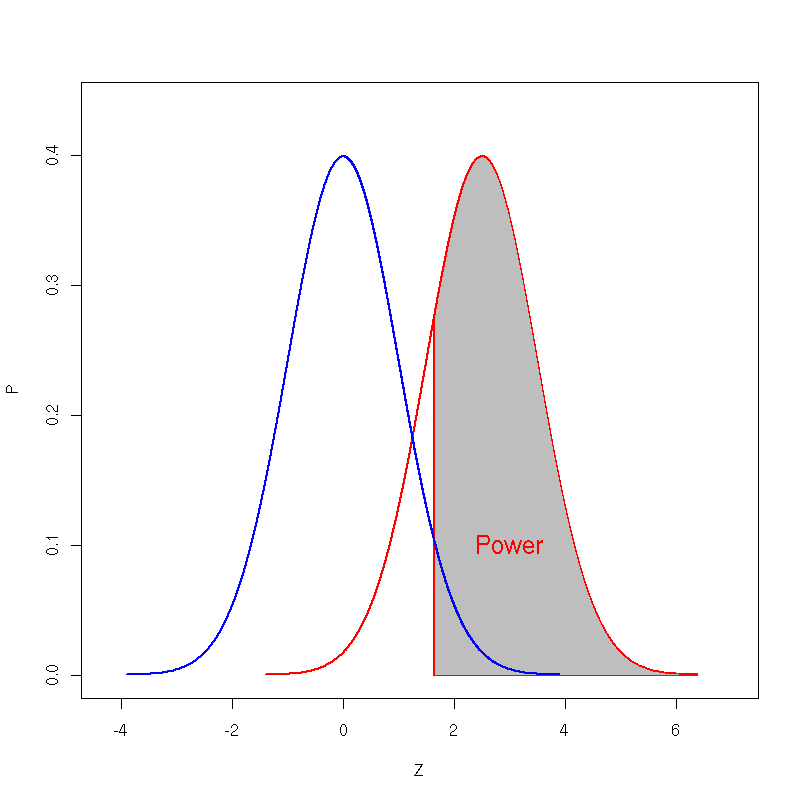
\includegraphics[scale=0.25]{Ztest.png}
  \end{center}
\end{frame}

\begin{frame}
  \vspace*{.5cm}
  The estimation of the Z-test power happens in this way:
  \vspace*{.25cm}
  \begin{itemize}
    \item The decision of the cut-off value $Z_{1-\alpha}$ or the standard normal distribution, valid for the null hypothesis;
    \item The calculation of the Z-distribution power valid when $ H_A $ is true, as area of this distribution not central at the right of the cut-off value $Z_{1-\alpha}$.
  \end{itemize}
\end{frame}

\begin{frame}
  From the expression of Z, it is deducible that Z increases. For this reason, the test should refuse the null hypothesis when the \textbf{difference} between the true mean $\mu$ and the hypothesized mean $\mu_0$ increases.
  \vspace*{.3cm}
  \begin{floatingfigure}[l]{5cm}
    \centering
    $\delta=2.5$\\
    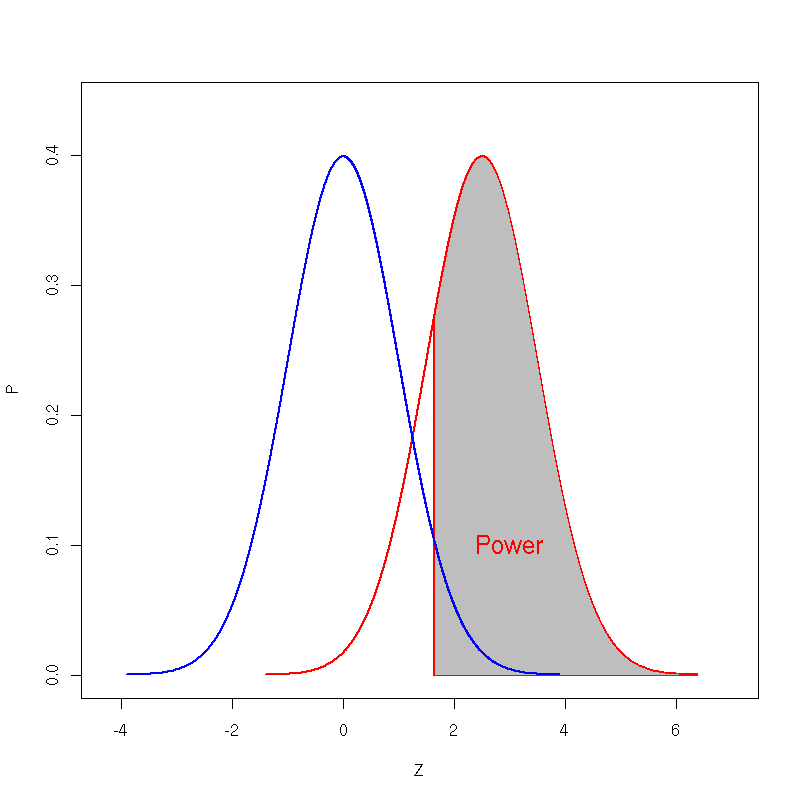
\includegraphics[scale=0.2]{Ztest1xm.png}\\
  \end{floatingfigure}
  \centering
  $\delta=3.5$\\
  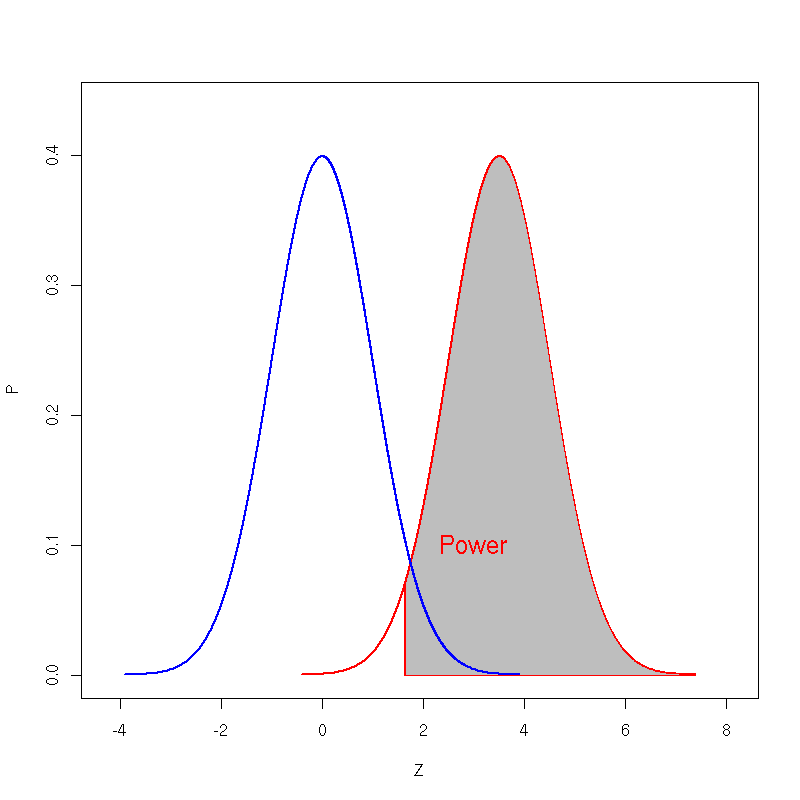
\includegraphics[scale=0.2]{Ztest2xm.png}\\
\end{frame}


\begin{frame}
  At the same time, when the value of $\sigma$ decreases, or the sample size {\boldmath $ n $} increases, the Z-value increases. For this reason, the power of the test to highlight a certain effect of dimension $\delta$ increases.\\
  \begin{floatingfigure}[l]{5cm}
    \centering
    $\sigma=3$\\
    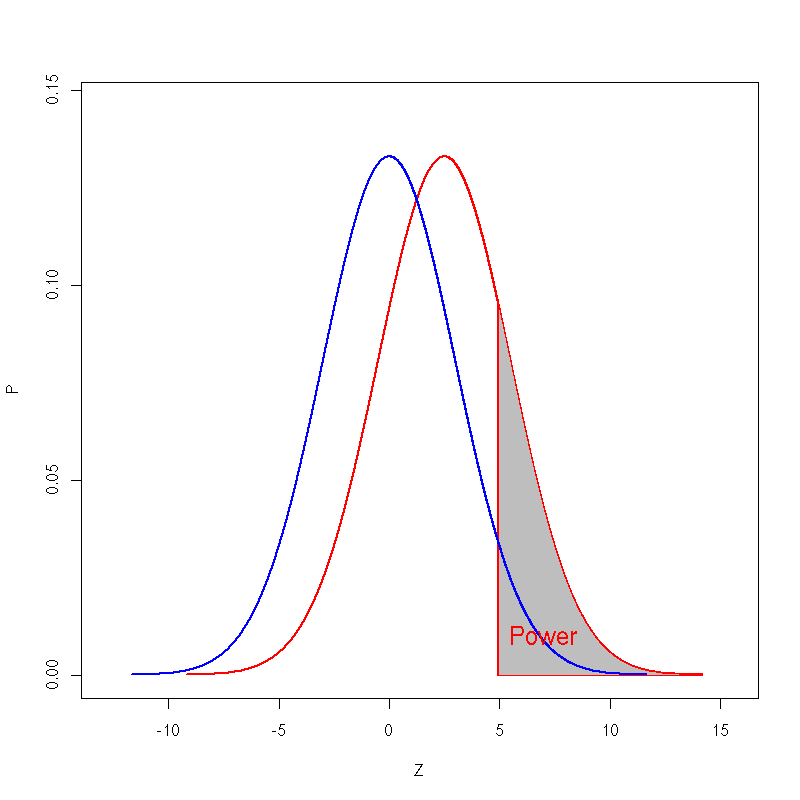
\includegraphics[scale=0.2]{Ztest2n.png}\\
  \end{floatingfigure}
  \centering
  $\sigma=1$\\
  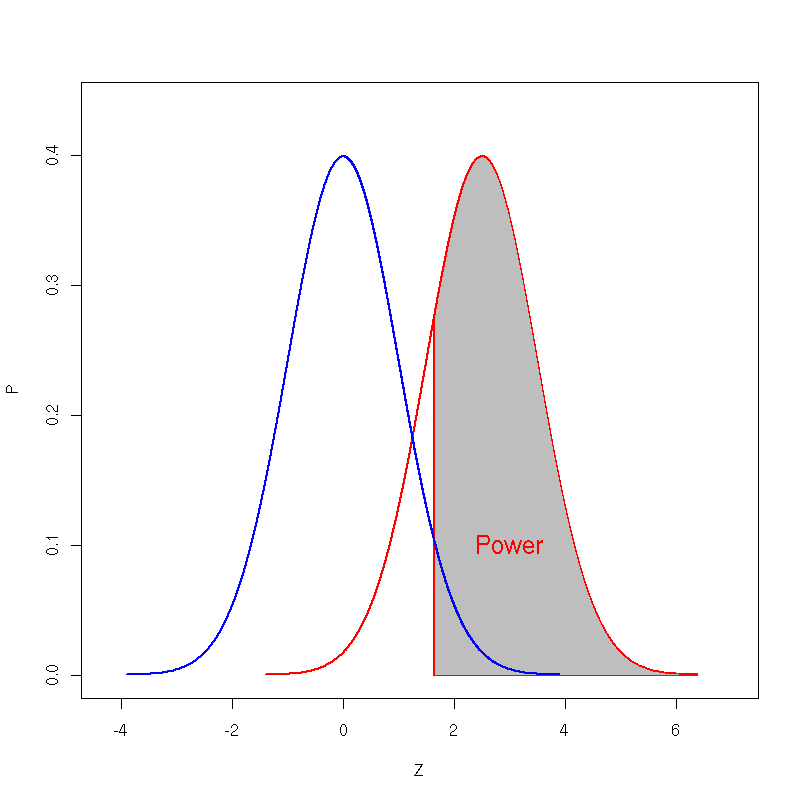
\includegraphics[scale=0.2]{Ztest1n.png}\\
\end{frame}

\begin{frame}
  \begin{small}
    Another aspect that influences the power of the test is the fact that the alternative hypothesis is \textbf{unilateral} or \textbf{bilateral}. This choice modifies the refusing area of the null hypothesis. With the same level of statistical significance $\alpha$, an unilateral test (picture on the left) is always more powerful of the correspondent bilateral test (picture on the right) as the critic value, upon which $H_0$ is refused, is smaller. The unilateral test is, without any doubts, preferable but it requires a larger quantity of preliminary information on the possible result of the test.
  \end{small}
  \begin{floatingfigure}[l]{5cm}
    \centering
    \vspace*{-4.3cm}
    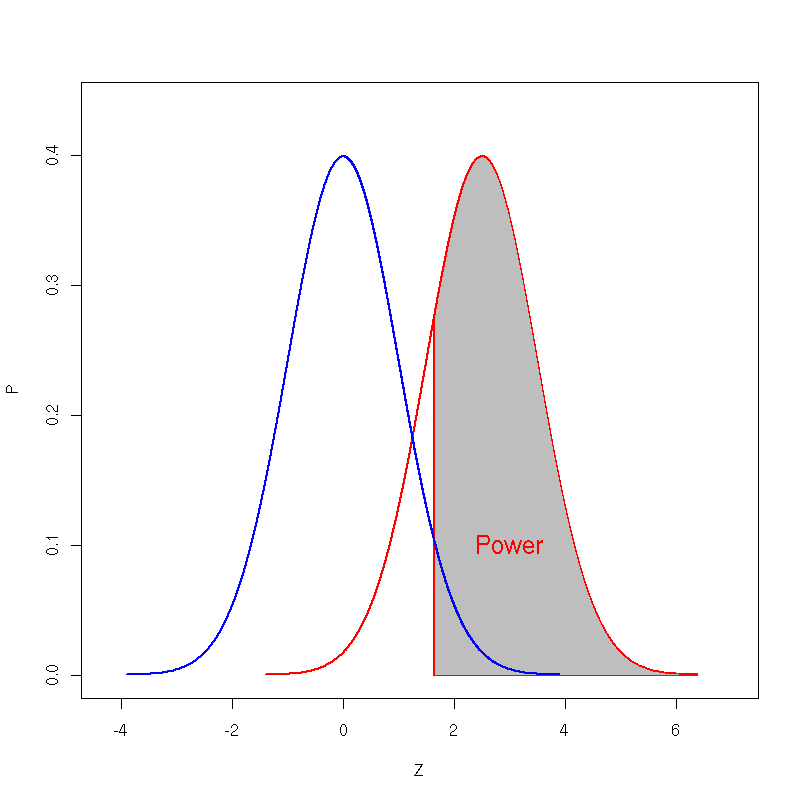
\includegraphics[scale=0.15]{ZtestUni.png}\\
  \end{floatingfigure}
  \vspace*{.3cm}
  \centering
  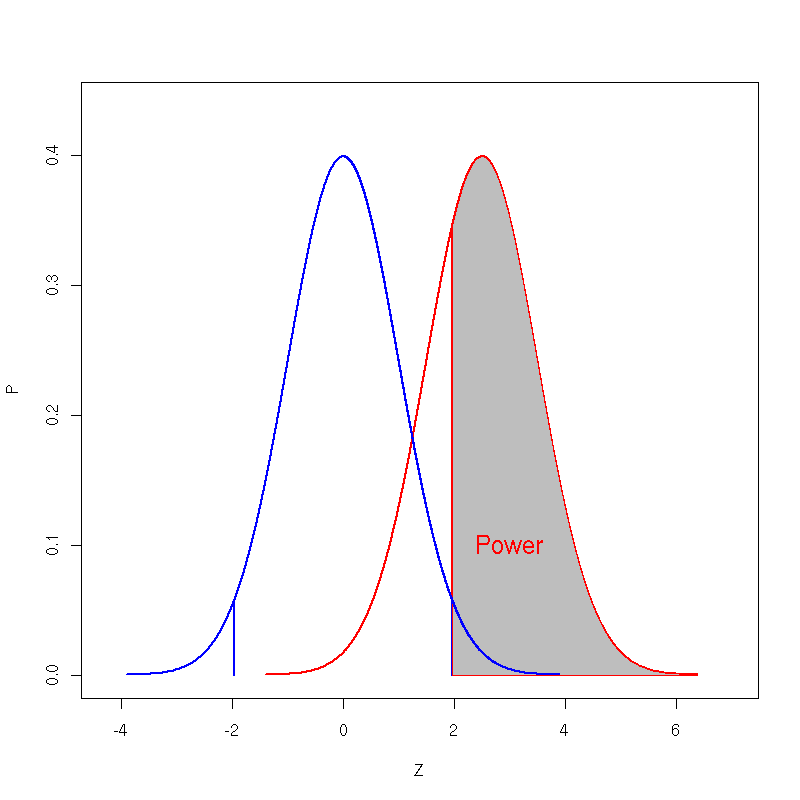
\includegraphics[scale=0.15]{ZtestBi.png}\\
\end{frame}

\livelloB{for the one sample t test or the paired two sample t test}

\begin{frame}
  \vspace*{.25cm}
  In the majority of the real cases, the \textbf{population variance is unknown} and the \textbf{use of}{\boldmath$s^2$} \textbf{instead of} {\boldmath$\sigma^2$} requires the use of the {\boldmath$t$} distribution in substitution of the Z-distribution.\\
  \vspace*{.5cm}
  When $ n $ is enough large, the Z-normal distribution and the t-distribution \textbf{are almost equal}. They provide similar answers. The differences are considered important when the sample has less than 30 observations and therefore the degrees of freedom of the t are a limited quantity.\\
  \vspace*{.5cm}
  Unlike the Z standard normal distribution, which is the unique, the \textbf{Student's t} distribution is a whole family of distributions, one for each value of degrees of freedom.
\end{frame}

\begin{frame}
  In these cases, the calculation of the three main parameters  ({\boldmath $ n $}, {\boldmath $ \delta $}, {\boldmath $ 1-\beta $}) is based on the same concepts, but with different formulas.\\
  \vspace*{.25cm}
  The analysis of the power and the calculation of the sample size is the same when the t-test is referred both to a \textbf{sample} and to two \textbf{dependent samples (paired)} because in this case it uses the column of the differences.\\
  \vspace*{.25cm}
  The t-test \textbf{power} is estimated:
  \begin{itemize}
    \item Calculating the cut-off value $ t_{1-\alpha,\nu} $ where $ \nu $ are the degrees of freedom of the t distribution, equal to {\boldmath $ n-1 $},
    \item And then establishing the area of t distribution valid with $ H_A $ at the right of the cut-off value:
    $$ t_{\beta,\nu} = \frac{\delta}{\sqrt{\frac{s^2}{n}}}-t_{\alpha,\nu} $$
\end{itemize}
\end{frame}

\begin{frame}
  \vspace*{.25cm}
  \begin{small}
    \textbf{t-distribution under the null hypothesis (at the left) and the alternative hypothesis (at the right) for the calculation of the power of the test.}
  \end{small}
  \begin{center}
    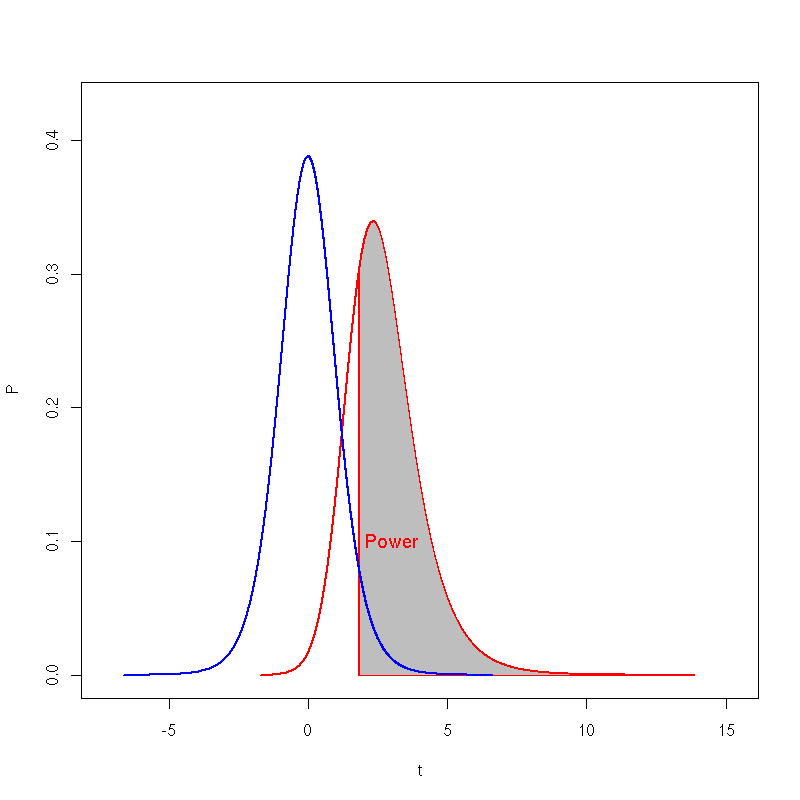
\includegraphics[scale=0.25]{Ttest.png}
  \end{center}
\end{frame}

\begin{frame}
  \begin{small}
    If it is necessary to establish, before collecting the data, how many observations are necessary to obtain or how many measures have to be done, for the estimation of  {\boldmath $ n $} it is used the following formula:
    $$ n\geq(t_{1-\alpha,\nu}+t_{\beta,\nu})^2\cdot \frac{s^2}{\delta^2}$$
    This formula depends on the two parameters $t_{1-\alpha,\nu}$ and $t_{\beta,\nu}$, which change according to the number of degrees of freedom {\boldmath$\nu$} and then (according to) the value of {\boldmath $ n $}.\\
%     \vspace*{.25cm}
    The calculation of {\boldmath $ n $} is done in an iterative way, starting from a first approximation (for example $ n=30 $ and then $\nu=29$). This statement makes the calculation of the quantiles $ t_{1-\alpha,\nu} $ and $ t_{\beta,\nu} $ possible. They are used in order to obtain a new estimation of {\boldmath $ n $}. If the calculated value is different from the initial value, new values of t, that correspond to the new estimation of {\boldmath $ n $}, are calculated. The value of {\boldmath $ n $} is then calculated again, until it is equal to the previous value (it is obtained by half up rounding {\boldmath $ n $} to its nearest integer because the number of observation cannot be, because of its nature, a decimal number).\\
  \end{small}
\end{frame}

\livelloB{for the two (independent) sample t test}

\begin{frame}
  \vspace*{.25cm}
  In a \textbf{t-test} for two samples \textbf{not matched}, or \textbf{independent}, the difference between the means of two samples is tested.\\
  \vspace*{.25cm}
  If the two samples are \textbf{balanced}, the test power is calculated with the same procedure of the t-test for one sample. The difference is that the number of df of the t-distribution has to be multiplied for 2 ($\nu=2n-2$):
  $$1-\beta=P\left( t_{(2n-2,\delta)}\geq t_{(1-\alpha,2n-2}\right)$$\\
  In this expression $t_{(1-\alpha,\nu)}$ is the quantiles of the central t distribution which corresponds to the cut-off value. $t_{(\nu,\delta)}$ is the non-central t distribution (with a non-centrality $\delta$ parameter), which is valid when the alternative hypothesis $ H_A $ is true. The probability that, with this distribution, the calculated statistics is at the right of the cut-off value, is the \textbf{power} {\boldmath$1-\beta$} of the test.
\end{frame}

\begin{frame}
  \vspace*{.5cm}
  When the two \textbf{samples are not balanced}, the calculation of the power happens in terms of the total sample size \textbf{N} and of the \textbf{weight} of the two independent samples ($\omega_1$ and $\omega_2$ proportions of the two different samples on the total sample size, with $\omega_1+\omega_2=1$):\\
  \vspace*{.5cm}
  $$ 1 - \beta = P \left (t_{(N-2,\delta)} \geq t_{(1-\alpha,N-2)} \right) $$
\end{frame}





\end{document}
